 %
% skript.tex -- Lecture notes for the PartDiff lectures given at the
%               MSE Master
%
% (c) 2006-2018 Prof. Dr. Andreas Mueller, HSR
%
\documentclass[a4paper,12pt]{book}
\usepackage[utf8]{inputenc}
\usepackage[T1]{fontenc}
%\usepackage{german}
\usepackage{times}
\usepackage{csquotes}
\usepackage{multirow}
\usepackage{subfigure}
\usepackage{geometry}
\usepackage{csquotes}
\geometry{papersize={210mm,297mm},total={160mm,240mm},top=31mm,bindingoffset=15mm}
\usepackage{amsmath}
\usepackage{amssymb}
\usepackage{amsfonts}
\usepackage{amsthm}
\usepackage{amscd}
\usepackage{graphicx}
\usepackage{fancyhdr}
\usepackage{textcomp}
\usepackage{txfonts}
\usepackage[all]{xy}
\usepackage{paralist}
%\usepackage[colorlinks=true]{hyperref}
\usepackage[pdfborder={0 0 0}]{hyperref}
\usepackage{array}
\usepackage{tikz}
\usepackage{pdfpages}

%für Querformat von zeitplan
\usepackage{pdflscape}

%für Abbreviations
\usepackage{acronym}

%figure float
\usepackage{float}

%für python code
\usepackage{listings}

%bibliography
\usepackage[hyperref=true,backend=biber,style=ieee,defernumbers=true]{biblatex}
\addbibresource{references.bib}

%%%%%%%%%%%%%%%%%%%%%%%
%% Copyleft
%% Walter A. Kehowski
%% Department of Mathematics
%% Glendale Community College
%% walter.kehowski@gcmail.maricopa.edu
%% \begin{linsys}{2}
%% -x & + & 4y & = & 8\\
%% -3x & - & 2y & = & 6
%% \end{linsys}
%%%%%%%%%%%%%%%%%%%%%%%
%\makeatletter
%% math-mode column types ------------------
\newcolumntype{\linsysR}{>{$}r<{$}}
\newcolumntype{\linsysL}{>{$}l<{$}}
\newcolumntype{\linsysC}{>{$}c<{$}}
\newenvironment{linsys}[1]{%
\begin{tabular}{*{#1}{\linsysR@{\;}\linsysC}@{\;}\linsysR}}%
{\end{tabular}}
%\makeatother
\endinput

\makeindex


\begin{document}
\pagestyle{fancy}
\lhead{}
\rhead{}
\frontmatter
\newcommand\HRule{\noindent\rule{\linewidth}{1.5pt}}



\hypersetup{
	colorlinks=true,
	linktoc=all,
	linkcolor=blue
}


\newtheorem{satz}{Theorem}[chapter]
\newtheorem{problem}[satz]{Problem}
\newtheorem{hilfssatz}[satz]{Lemma}
\newtheorem{definition}[satz]{Definition}
\newtheorem{annahme}[satz]{Assumption}
\newtheorem{aufgabe}[satz]{Task}
\newenvironment{beispiel}[1][Example]{%
	\begin{proof}[#1]%
		\renewcommand{\qedsymbol}{$\bigcirc$}
	}{\end{proof}}
%\allowdisplaybreak


\begin{titlepage}
\vspace*{\stretch{1}}
\HRule
\vspace*{10pt}
\begin{flushright}
{\LARGE
Fast Computer Vision based Geometry Estimation}

%\Large{with Rotation, GPS and On-Board-Diagnostics Sensor Data}
\end{flushright}
\begin{flushright}
{\Large Bachelor Thesis}
\end{flushright}
\HRule

\vspace{70pt}
\large
\textbf{Authors}

Cédric Renda, Manuel Tischhauser

\textbf{Supervisor}

Prof. Dr. Guido M. Schuster 

\textbf{Subject}

Image Processing



\vspace*{\stretch{2}}
\begin{center}
HSR Hochschule Für Technik Rapperswil

\today
\end{center}
\end{titlepage}


\chapter*{Abstract}

\section*{Introduction}
Mass production in the industry requires a periodical check of quality and dimensions of each part in different stations of the production chain.
In the special case of this thesis, the object to be measured is a steel spring.
Until today the spring has to be measured by hand by a production worker. In a production chain with a capacity of 200 springs per minute only some few springs actually get measured.
With conventional methods it s hard to get an accurate measurement because of the geometry of the spring and even harder to make these measurements reproducible because of the elasticity of the used steel.

This two difficulties can be solved by using cameras to estimate the geometry.
But such cameras and lenses suitable for such tasks are in many cases simply to expensive.

\section*{Approach}
It should be possible to compensate the flaws of a low-cost hardware by the software running on a platform with high computing power.
The software has to take into account and correct all the imperfections of the lens while at the same time manage to execute these task fast enough so the whole setup can be placed in the production chain.
Instead of making periodic measurements, it should this way be possible to estimate the geometry of every passing object.

In the case of the steel spring, the setup should be able to make accurate measurements (relative error = standard deviation/mean > 1\%).
With 200 springs per minute the setup has therefore to handle about 4 geometry estimations per second to be on the safe side.

Over the course of this thesis, a demonstrator, using a Raspberry Pi Camera Module V2, has been developed.
To demonstrate measurements performed on a moving object, the steel springs can be sidled over a tilted glass plate mounted in front of a backlight.
The camera is mounted parallel to the glass plate.
The software detects if a object moves through the field of view of the camera and measures the length and diameter.
These tasks are performed on a Nvidia Jetson Nano developer kit.

\section*{Conclusion}
In the static case, it was possible to achieve a relative error in the length of 0.22\% and in the diameter of 0.55\%.
With an object sliding with at an estimated speed of 2\,m/s over the glass plate, a relative error of 1.01\% in the length and 1.60\% in the diameter could be achieved.
The trigger checks for object in image with 21\,fps and the calculations can be performed at a rate of 15\,fps. 

\tableofcontents

\mainmatter

\chapter*{Abbreviations}
\addcontentsline{toc}{chapter}{Abbreviations} 
%A
\begin{acronym}
	\acro{rms}[RMS]{Root Mean Square}
\end{acronym}









\chapter{Introduction}
Production chains in the industry require a periodical measurement of the dimensions of the produced part.
If the measured values deviate to much from the desired value, the production has to be adjusted in order to keep the quality of the part.
In much cases this is done by a production worker who takes a random sample of produced parts and supervises this way the whole manufacturing process.

This thesis focuses on the manufacturing of steel springs.
Since the geometry of such a spring is rather complex, it is rather difficult to make a good measurement with conventional methods (e.g. manually).
Additionally, the elasticity of the steel makes it even more difficult to reproduce the measurements.

Estimating the geometry of the spring from the images taken by a camera mounted in the production chain could solve this problem, but optics used for measurements are usually too expensive.
Additionally, it would be very helpful to use multiple setups distributed over the whole production chain to determine in which production-step an error occurred.
This increases the cost for such a measurement device even more.
Since computing power is nowadays very cheap, these costs could be lowered dramatically by using a low-cost camera and compensating the cheap hardware with the software.

In this bachelor thesis, a device, called the demonstrator, has been developed to demonstrate the working principle of this setup.
In the first chapter the task analysis and approach will be evaluated.
The second chapter focuses on the general theory applied in the development.
The development itself will be described in more detail in Chapter three.
The fourth chapter discusses the results, followed by the conclusion in the sixth chapter. 

\newpage
\section{Task analysis}
The primary goal of this bachelor thesis was to develop a working demonstrator in order to show, that it really is feasible to make this kind of measurements with a low-cost device.
The demonstrator should be able to make measurements of length and diameter of the spring with a relative error (standard deviation/mean) of less than 1\%.
Since it is expected, that the production manufactures 200 springs per minute, the software which makes the necessary corrections an estimates the dimensions has to make about four measurements per second to be on the safe side.

\section{Approach}
It is reasonable to split this task into a hardware and a software part.

\subsection{Hardware}
The hardware consists of the following parts:
\begin{itemize}
	\item Raspberry Pi Camera Module V2
	\item Nvidia Jetson Nano developer kit
	\item Backlight illumination
	\item Mechanical construction
\end{itemize}
The Pi Camera Module delivers an image stream to the Jetson Nano where all the computing takes place.
To make the handling of the image easier, the spring is lit from the back with a specially designed illumination.
This makes it possible to threshold the incoming frames to a binary image, on which it is much easier (and faster) to operate on.
A mechanical construction consisting mainly of aluminum profiles serves as a framwork on which all other components can be attached.

\subsection{Software}
To compensate lens imperfections, the camera has to be calibrated and this has to be done for every camera once before using it.
The software later uses the results from the calibration to adjust the image.
A software trigger checks all the frames for the a passing object.
If it found such a frame it passes this image to the next section of the software which is responsible for following tasks:
\begin{itemize}
	\item Undistort the image using the results from the calibration
	\item Find a known pattern on the plane as reference
	\item Transform the image to correct a tilted view of the camera to the plane
	\item find the Object (spring) in the frame
	\item Estimate the geometry (length and diameter) of the object
\end{itemize} 


\chapter{Theory}\label{theory}
This chapter takes a closer look at the theory and technology applied in this thesis.

\section{Camera Calibration in OpenCV}
Camera calibration is needed to obtain camera parameters like focal length and center point.
Further, it provides a method to correct distortions caused by the imperfect optics according to a certain distortion models.
For that, a set of images of a known pattern (usually a checkerboard) have to be taken from different view-points an angles.
These points provide the training data which is needed to estimate all the coefficients.

This section describes the theory behind the calibration process in OpenCV 4.3.0, which is the latest version at the time of writing this thesis.
\subsection{The pinhole camera model}
The functions OpenCV provides to calibrate the camera use the so-called pinhole camera model \cite{cv_calib}.
This model describes, how a 3D-point specified in world-coordinates ($P_w$) is transformed to a 3D-point in camera-coordinates ($P_c$) and then further projected onto the image plane ($p$). After this step, the point is described as a 2D-point in pixel coordinates.  Figure \ref{theory:pin} illustrates this setup.
\begin{figure}[ht]
	\centering
	%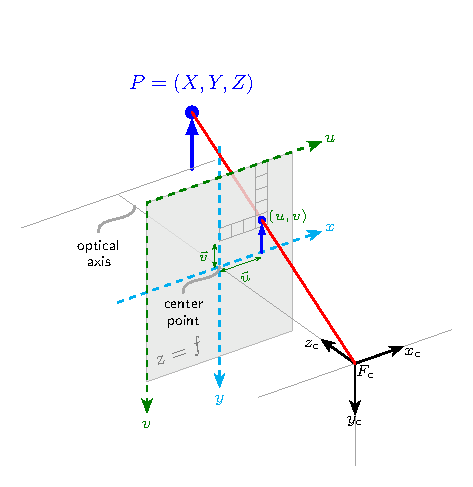
\includegraphics[width=0.9\textwidth]{2-theory/camera/camera.pdf}
	\caption{Pinhole-model (not up to date).\label{theory:pin}}
\end{figure} 

The transition from the world-coordinates to the camera-coordiantes can be described as 
\begin{align*}
\underbrace{\begin{pmatrix}
X_c\\
Y_c\\
Z_c\\
\end{pmatrix}}_{P_c}=
\underbrace{\begin{pmatrix}
r_{11}&r_{12}&r_{13}\\
r_{21}&r_{22}&r_{23}\\
r_{31}&r_{32}&r_{33}
\end{pmatrix}}_{R}
\underbrace{\begin{pmatrix}
X_w\\
Y_w\\
Z_w\\
\end{pmatrix}}_{P_w}+
\underbrace{\begin{pmatrix}
t_x\\
t_y\\
t_z\\
\end{pmatrix}}_{t}.
\end{align*}
The vector $P_w$ is first rotated by $R$ and the translated by $t$. This can be written in one single matrix:
\begin{align}
\begin{pmatrix}
X_c\\
Y_c\\
Z_c
\end{pmatrix}=
\begin{pmatrix}
r_{11}&r_{12}&r_{13}&t_x\\
r_{21}&r_{22}&r_{23}&t_y\\
r_{31}&r_{32}&r_{33}&t_z
\end{pmatrix}
\begin{pmatrix}
X_w\\
Y_w\\
Z_w\\
1
\end{pmatrix}\quad\Leftrightarrow\quad
P_c=
\begin{pmatrix}
R&|&t
\end{pmatrix}
\begin{pmatrix}
P_w\\
1
\end{pmatrix}\label{theory:world-camera}.
\end{align}

As a result of the theorem of intersecting lines, the projection from $P_c$ to $p$ is described as
\begin{align*}
\underbrace{\begin{pmatrix}
u\\
v
\end{pmatrix}}_{p}=
\begin{pmatrix}
f_x\cdot X_c/Z_c\\
f_y\cdot y_c/Z_c\\
\end{pmatrix}+
\begin{pmatrix}
c_x\\
c_y
\end{pmatrix}.
\end{align*}
where $f_x$ and $f_y$ are the focal length $f$ (in world units) normalized by their respective pixel size (in world units). Thus $f_x$ and $f_y$ are the same, if the pixels are quadratic.

By adding the principal point $\begin{pmatrix}c_x&c_y\end{pmatrix}^T$, which is usually close to the image center, it is taken into account, that pixel-coordinates are specified with respect to the upper left corner of the image plane. .
It is now simpler to write this in homogeneous coordinates:
\begin{align}
\begin{pmatrix}
u\\
v\\
1
\end{pmatrix}\sim s
\begin{pmatrix}
u\\
v\\
1
\end{pmatrix}=
\underbrace{\begin{pmatrix}
f_x&0&c_x\\
0&f_y&c_y\\
0&0&1
\end{pmatrix}}_{K}
\begin{pmatrix}
X_c\\
Y_c\\
Z_c
\end{pmatrix}\quad \Leftrightarrow \quad s
\begin{pmatrix}
p\\
1
\end{pmatrix}=
K\cdot P_c
\label{theory:camera-pixel},
\end{align}
where $s$ is an arbitrary scaling factor and $K$ is called the camera matrix.
The overall transition from world- to pixel-coordinates is the result of combining \ref{theory:world-camera} and \ref{theory:camera-pixel}:
\begin{align}
s
\begin{pmatrix}
u\\
v\\
1
\end{pmatrix}=
\begin{pmatrix}
f_x&0&c_x\\
0&f_y&c_y\\
0&0&1
\end{pmatrix}
\begin{pmatrix}
r_{11}&r_{12}&r_{13}&t_x\\
r_{21}&r_{22}&r_{23}&t_y\\
r_{31}&r_{32}&r_{33}&t_z
\end{pmatrix}
\begin{pmatrix}
X_w\\
Y_w\\
Z_w\\
1
\end{pmatrix}\quad \Leftrightarrow \quad s
\begin{pmatrix}
p\\
1
\end{pmatrix}=
K
\begin{pmatrix}
R&|&t
\end{pmatrix}
\begin{pmatrix}
P_w\\
1
\end{pmatrix}\label{theory:world-pixel}
\end{align}
The rotation and translation in $\begin{pmatrix}R&|&t\end{pmatrix}$ are called the extrinsic parameters. The camera matrix $K$ contains analogously the linear intrinsic parameters.

\subsection{The distortion model in OpenCV}
Non linear distortions, which appear before the projection in \ref{theory:camera-pixel} should be considered too.
OpenCV takes the effects of radial, tangential and thin prism distortion into account \cite{cv_calib}. 

\subsubsection{Radial Distortion}
Radial distortion is caused by the flawed curvature of the lens \cite{weng}.
It can be modeled with
\begin{align}
\begin{pmatrix}
x''\\
y''
\end{pmatrix}=
\begin{pmatrix}
x'\frac{1+k_1 r^2+k_2 r^4+k_3 r^6}{1+k_4 r^2+k_5r^4+k_6r^6}\\
y'\frac{1+k_1 r^2+k_2 r^4+k_3 r^6}{1+k_4 r^2+k_5r^4+k_6r^6}
\end{pmatrix}\label{theory:raddist},
\end{align}
where $x'$ and $y'$ are coordinates, described in camera-coordinates, normalized with $Z_c$
\begin{align*}
\begin{pmatrix}
x'\\
y'
\end{pmatrix}=
\begin{pmatrix}
X_c/Z_c\\
Y_c/Z_c
\end{pmatrix}
\end{align*}from
and r is the radius as taken with respect to the principal point $\begin{pmatrix}c_x&c_y\end{pmatrix}^T$
\begin{align*}
r^2 = x'^2 + y'^2.
\end{align*}
This type of distortion is symmetrical about the optical axis.
Figure \ref{theory:radial} illustrates the effect on a rectangle.
\begin{figure}[ht]
	\centering
	\includegraphics[width=0.9\textwidth]{2-theory/distortion/radial.png}
	\caption{Different types of radial distortion. Black: no distortion, red: $k_1 = 10$, $k_2=11$, $k_3=12$, $k_4=5$, $k_5=6$, $k_6=7$, blue: $k_1 = -2.2$, $k_2=-1.2$, $k_3=-0.8$, $k_4=-0.4$, $k_5=-0.3$, $k_6=-0.2$\label{theory:radial}}
\end{figure} 

\subsubsection{Tangential distortion}
Real optical systems are also subject to tangential distortion. This type of distortion has a decentering effect and occurs, if the line through the optical center of the lens and the principal point is not col-linear with the optical axis \cite{weng}.
The model
\begin{align}
\begin{pmatrix}
x''\\
y''
\end{pmatrix}=
\begin{pmatrix}
x' + 2p_1x'y'+p_2(r^2+2x'^2)\\
y' + 2p_2x'y'+p_1(r^2+2y'^2)
\end{pmatrix}\label{theory:tandist}
\end{align}
takes this into account.
Figure \ref{theory:tangential} shows the distortion this model introduces.

\begin{figure}[ht]
	\centering
	\includegraphics[width=0.9\textwidth]{2-theory/distortion/tangential.png}
	\caption{Different types of tangential distortion. Black: no distortion, red: $p_1 = -0.15$, $p_2=-0.4$, blue: $p_1 = 0.15$, $p2=-0.4$\label{theory:tangential}}
\end{figure} 

\subsubsection{Thin prism distortion}
Thin prism distortion is partially caused by lens imperfections and camera assembly \cite{weng}.
It introduces additional radial and tangential distortion, modeled with
\begin{align}
\begin{pmatrix}
x''\\
y''
\end{pmatrix}=
\begin{pmatrix}
x' + s_1 r^2 + s_2 r^4\\
y' + s_3 r^2 + s_4 r^4
\end{pmatrix}\label{theory:prismdist}.
\end{align}

\subsubsection{The combined model in OpenCV}
The models in \ref{theory:raddist}, \ref{theory:tandist} and \ref{theory:prismdist} combined result in
\begin{align}
\begin{pmatrix}
x''\\
y''
\end{pmatrix}=
\begin{pmatrix}
x'\frac{1+k_1 r^2+k_2 r^4+k_3 r^6}{1+k_4 r^2+k_5r^4+k_6r^6}+2p_1 x' y'+p_2(r^2+2x'^2)+s_1 r^2+s_2 r^4\\
y'\frac{1+k_1 r^2+k_2 r^4+k_3 r^6}{1+k_4 r^2+k_5r^4+k_6r^6}+2p_2x'y'+p_1(r^2+2y'^2)+s_3 r^2+s_4 r^4
\end{pmatrix}\label{theory:dist}.
\end{align}
In summary, a point in normalized camera-coordinates $\begin{pmatrix}x'&y'\end{pmatrix}^T$ is distorted as modeled in \ref{theory:dist}, which leads to the point $\begin{pmatrix}x''&y''\end{pmatrix}^T$. To get the distorted pixel-coordinates (subscript $d$), the projection has to be applied
\begin{align*}
\begin{pmatrix}
u_d\\
v_d\\
\end{pmatrix}=
\begin{pmatrix}
x''f_x+c_x\\
y''f_y+c_y
\end{pmatrix}\quad\Leftrightarrow\quad
\begin{pmatrix}
u_d\\
v_d\\
1
\end{pmatrix}=K
\begin{pmatrix}
x''\\
y''\\
1
\end{pmatrix},
\end{align*}
which completes the model so far.
Keep in mind, that when correcting the distortion, equation \ref{theory:dist} has to be inverted.

\subsection{Reprojection error}
The reprojection error is a value to asses the quality of a calibration.
It is the error between the detected image point and the projection (using the obtained coefficients) of its corresponding world point onto the image plane.
Since it only uses the points, which where previously used to obtain the calibration-parameters, it can be interpreted as a training error rate.

Calibration functions in OpenCV return the overall \acs{rms} reprojection error \cite{cv_calib}.

\subsection{Error propagation as further quality assessment}
As argued before, the reprojection error is a training error rate.
A low reprojection error is therefore not necessarily enough to estimate, how good the calibration really performs.

OpenCV returns with its extended calibration functions not only the camera intrinsics, but also an estimated standard deviation of each coefficient \cite{cv_calib}.
Under assumption that low standard deviations suggest a good calibration, it is valid to combine all standard deviations into one value using the propagation of uncertainty.

The propagation of error states that influence of each error of the inputs $x_i$ on the output value $y$ of a function
\begin{align*}
	y = f(x_1, x_2,..,x_n)
\end{align*}
can be linearly approximated and summed up to:
\begin{align}
	\Delta y = \sqrt{\sum_{i=1}^{n}\left(\frac{\partial y}{\partial x_i}\Delta x_i \right)^2} \label{theory:prop}.
\end{align}

Applied to \ref{theory:dist}, this leads to
\begin{align*}
	\Delta x''=\sqrt{\sum_{i=1}^{6}\left(\frac{\partial x''}{\partial k_i}\Delta k_i \right)^2+\sum_{i=1}^{2}\left( \frac{\partial x''}{\partial p_i}\Delta p_i\right)^2+\sum_{i=1}^{4}\left( \frac{\partial x''}{\partial s_i}\Delta s_i\right)^2}
\end{align*}
and
\begin{align*}
	\Delta y''=\sqrt{\sum_{i=1}^{6}\left(\frac{\partial y''}{\partial k_i}\Delta k_i \right)^2+\sum_{i=1}^{2}\left( \frac{\partial y''}{\partial p_i}\Delta p_i\right)^2+\sum_{i=1}^{4}\left( \frac{\partial y''}{\partial s_i}\Delta s_i\right)^2}.
\end{align*}
It is at this point not intended to go into further computations of the derivatives.
If we look at pixel coordinates from the center of the image, btw. $c_x=0$ and $c_y=0$, the radius (distance from the centerpoint) can be expressed as
\begin{align*}
	r = \sqrt{(f_x\cdot x'')^2+(f_y\cdot y'')^2}
\end{align*}
and therefore, if errors in $f_x$ and $f_y$ are neglected, with the propagation in \ref{theory:prop} applied
\begin{align}
	\Delta r = \sqrt{\left(\frac{\partial r}{\partial x''} \Delta x''\right)^2+\left(\frac{\partial r}{\partial y''} \Delta y''\right)^2}\label{theory:delta_r}.
\end{align}
This value $\Delta r$ can now be plotted over half the diagonal of an image to compare calibration coefficients of different calibration approaches.



\section{Measurement with back-light illumination}
To measure the size and form of an object there are multiple ways. A popular way to get the contour is to place a light source behind the object desired to measure, and aim on the object with an camera. With this method the optical sensors get the silhouette of the object. 
\subsection{Short introduction to photometry}
Photometry is the science concerned with the electromagnetic radiation visible to the human eye. In this section some important basics used further in this paper are explained. The theories of the following sections were taken from the textbook Physik 2 \cite{ruh}
\subsubsection{Photometric quantities}
In principle the normal physical quantities and units such as watts and joules could be used for the measurements of light radiation. However, in order to take into account the spectral sensitivity of the human eye, special photometric quantities and units are introduced.\\

\begin{table}[ht]
\centering
\begin{tabular}{ |p{5cm} p{2cm}|p{5cm} p{2cm} p{2cm}|  }
	\hline
	\multicolumn{2}{|c}{Quantity}&\multicolumn{3}{|c|}{Unit} \\
	\hline\hline
	\multicolumn{1}{|c}{Name}			& \multicolumn{1}{|c|}{Symbol}	& \multicolumn{1}{c}{Name}	& \multicolumn{1}{|c|}{Symbol}	& \multicolumn{1}{|c|}{SI-unit}\\

	\hline
	Luminous flux		& \multicolumn{1}{|c|}{$\phi_v$}	& lumen		& \multicolumn{1}{|c|}{lm}& \multicolumn{1}{|c|}{W}\\
	Luminous intensity 	& \multicolumn{1}{|c|}{$I_v$} 		& candela	& \multicolumn{1}{|c|}{cd}& \multicolumn{1}{|c|}{W/sr}\\
	Luminance			& \multicolumn{1}{|c|}{$L_v$}		& candela/$\text{m}^2$	& \multicolumn{1}{|c|}{cd/$m^2$}& \multicolumn{1}{|c|}{W/$\text{m}^2$sr}\\
	Illuminace 			& \multicolumn{1}{|c|}{$E_v$} 		& lux (=lumen/$\text{m}^2$) 	& \multicolumn{1}{|c|}{lx}& \multicolumn{1}{|c|}{W/$\text{m}^2$}\\

	\hline
\end{tabular}
\end{table}


Luminous intensity or candela is the Luminous flux per unit solid angle. It describes the perceived power per unit solid angle. As example we assume to have a light with a 10 lumen strong light source. If the light beam is now focused into 1 steradian light beam, the beam would be 10 candela.\\
Luminace is used 
\begin{align*}
L_{\mathrm{v}}=\frac{\mathrm{d}^{2} \Phi_{\mathrm{v}}}{\mathrm{d} \Sigma \mathrm{d} \Omega_{\Sigma} \cos \theta_{\Sigma}}
\end{align*}


\subsubsection{Light source}
To model a light source it is assumed that the source is a very small point which emits the light rays in all directions and is measured in luminous flux. The density of the light rays is reduced with the factor $\frac{1}{r^2}$ with $r$ being the distance. Luminous intensity of the light is proportional to the density of the rays. This behavior has to do with the fact that the surface area $A$ of a sphere
\begin{align*}
A=\int_{0}^{2 \pi} \int_{0}^{\pi} r^{2} \sin \theta d \theta d \varphi=4 \pi r^{2}
\end{align*}
grows squared with the distance from the center $r$.
\begin{align*}
A = 4\pi r^2
\end{align*}
In photometry the usage of solid angle is very common.  
\begin{figure}[ht]
	\centering
	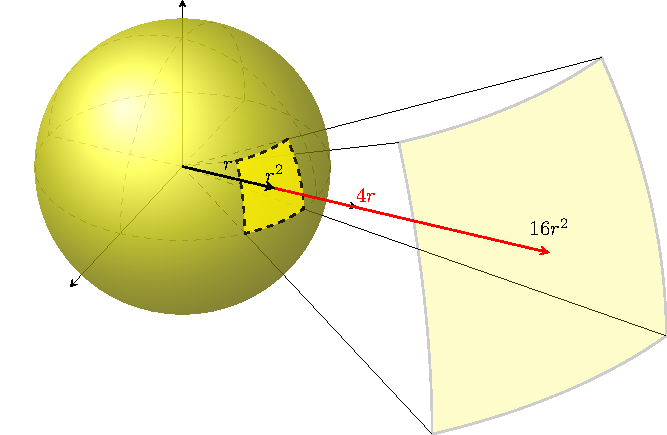
\includegraphics[width=0.6\textwidth]{2-theory/backlight/light.pdf}
	\caption{Light source in 3d\label{theory:light}}
\end{figure} 
\\

\subsubsection{Luminous flux}
Luminous flux or lumen is Luminous flux per unit time and has the unit candela steradians ($cd\cdot sr$). It is used to describe the total amount of light a lamp puts out. The 
\begin{table}[ht]
	\centering
	\begin{tabular}{ |p{5cm} p{2cm}|p{5cm} p{2cm} p{2cm}|  }
		\hline
		\multicolumn{2}{|c}{Quantity}&\multicolumn{3}{|c|}{Unit} \\
		\hline\hline
		\multicolumn{1}{|c}{Name}			& \multicolumn{1}{|c|}{Symbol}	& \multicolumn{1}{c}{Name}	& \multicolumn{1}{|c|}{Symbol}	& \multicolumn{1}{|c|}{SI-unit}\\
		
		\hline
		Luminous flux		& \multicolumn{1}{|c|}{$\phi_v$}	& lumen		& \multicolumn{1}{|c|}{lm}& \multicolumn{1}{|c|}{W}\\
		Luminous intensity 	& \multicolumn{1}{|c|}{$I_v$} 		& candela	& \multicolumn{1}{|c|}{cd}& \multicolumn{1}{|c|}{W/sr}\\
		Luminance			& \multicolumn{1}{|c|}{$L_v$}		& candela/$\text{m}^2$	& \multicolumn{1}{|c|}{cd/$m^2$}& \multicolumn{1}{|c|}{W/$\text{m}^2$sr}\\
		Illuminace 			& \multicolumn{1}{|c|}{$E_v$} 		& lux (=lumen/$\text{m}^2$) 	& \multicolumn{1}{|c|}{lx}& \multicolumn{1}{|c|}{W/$\text{m}^2$}\\
		
		\hline
	\end{tabular}
\end{table}


\lipsum[4]\\





\chapter{Development}
This chapter covers the developing process in more detail.

\section{Hardware}
In this chapter we give a short oversight what hardware is used and how big the price tag of the demonstrator is. 

\subsection{Computer}
The computer used is the Nvidia Jetson Nano developer kit.
A short technical overview is listed in Table \ref{development:nano}.
\begin{table}[ht]
	\begin{tabular}{|l|l|}
		\hline
		\multicolumn{2}{|c|}{Technical specifications of the Jetson Nano} \\
		\hline
		GPU			& 	128-core Maxwell\\
		CPU			& 	Quad-core ARM A57 @ 1.43 GHz \\
		Memory 		&	4 GB 64-bit LPDDR4 25.6 GB/s 				\\
		Storage		&	microSD				\\
		Video Encode&	4K @ 30 | 4x 1080p @ 30 | 9x 720p @ 30 (H.264/H.265) \\
		Video Decode&	4K @ 60 | 2x 4K @ 30 | 8x 1080p @ 30 | 18x 720p @ 30 (H.264/H.265) \\
		Camera 		&	2x MIPI CSI-2 DPHY lanes \\
		Connectivity&	Gigabit Ethernet, M.2 Key E\\
		Display 	&	HDMI and display port \\
		USB 		&	4x USB 3.0, USB 2.0 Micro-B\\
		Others 		&	GPIO, I2C, I2S, SPI, UART \\
		Mechanical 	&	69 mm x 45 mm, 260-pin edge connector \\		
		\hline
	\end{tabular}
	\caption{Jetson Nano specifications \cite{jetson}.\label{development:nano}}
\end{table}


\subsection{Camera}
The camera used for this project had to following evaluation criteria to meet:
\begin{itemize}
	\item Compatible with the Jetson Nano enviroment
	\item A good developer community
	\item Open source drivers
	\item Low cost
\end{itemize}

Table \ref{development:cameras} lists some of the cameras that have been evaluated for the project.
\begin{table}[ht]
	\centering
	\begin{tabular}{ |l||c|c|c|  }
		\hline
		\multicolumn{4}{|c|}{List of possible Cameras} \\
		\hline\hline
		Company				& Raspberry Pi 		& Raspberry Pi	& Arducam\\
		Camera Name			& Camera Module V2 	& HQ Camera		& Arducam IMX219 \\
		&					&				&Low Distortion M12 \\
		&					&				&Mount Camera Module\\
		\hline
		Price				& \$25 				& \$50  		& \$39.99 \\
		Camera Sensor   	& Sony IMX219 		& Sony IMX477	& Sony IMX219\\
		
		Still resolution	& 8M 				& 12M			& 12.3M\\
		Sensor resolution 	& 3280 x 2464 		& 4056 x 3040 	& 3280 x 2464\\
		Linux integration   & V4L2 driver 		& V4L2 driver	& V4L2 driver\\
		Pixel size			& 1.12 x 1.12 $\mu\text{m}$	& 1.55 x 1.55$\mu\text{m}$ & 1.12 x 1.12 $\mu\text{m}$ \\
		Focal length		& 3.04$[\text{mm}]$ & Depends on lens & 2.8$[\text{mm}]$\\
		Focal ratio			& 2.0  				& Depends on lens & 2.8\\
		View angle Horizontal & 62.2 deg.		& Depends on lens & 75 deg.\\
		\hline
	\end{tabular}
\caption{List of suitable cameras.\label{development:cameras}}	
\end{table}

In the end, all results were measured with the Raspberry Pi Camera Module V2 since it was the cheapest one in the list and seems to deliver the desired results.

\subsection{Backlight}
The main component of the backlight is a PCB.
In front of the PCB there are three stacked glass plates, on which diffusion filters and the geometry pattern later used for the measurements can be attached.
This is shown in Figure \ref{development:glass}.
\begin{figure}[ht]
	\centering
	\setlength{\tabcolsep}{12em}
	{\renewcommand{\arraystretch}{1}	
	\begin{tabular}{|c|}
		\hline
		\multicolumn{1}{|c|}{glass (2\,mm)}\\
		\hline
		\multicolumn{1}{|c|}{geometry pattern}\\
		\hline
		\multicolumn{1}{|c|}{glass (2\,mm)}\\
		\hline
		\multicolumn{1}{|c|}{diffusion filter}\\
		\hline
		\multicolumn{1}{|c|}{glass (2\,mm)}\\
		\hline
	\end{tabular}
	}
	\caption{Stacked glass plates.\label{development:glass}}
\end{figure}

The geometry pattern consists of five black squares in two rows.
The PCB is equipped with 39 LEDs an used two times.
One LED has a luminious flux of 76\,lm @ 4000\,K 80\,CRI \cite{led}.
The backlight should therefore have a total luminious flux of 5928\,lm.
The whole backlight consumes ca. 12\,A at 5\,V which corresponds to a total power consumption of 60\,W. 

The PCB is shown in Figure \ref{development:pcb}.
\begin{figure}[ht]
	\centering
	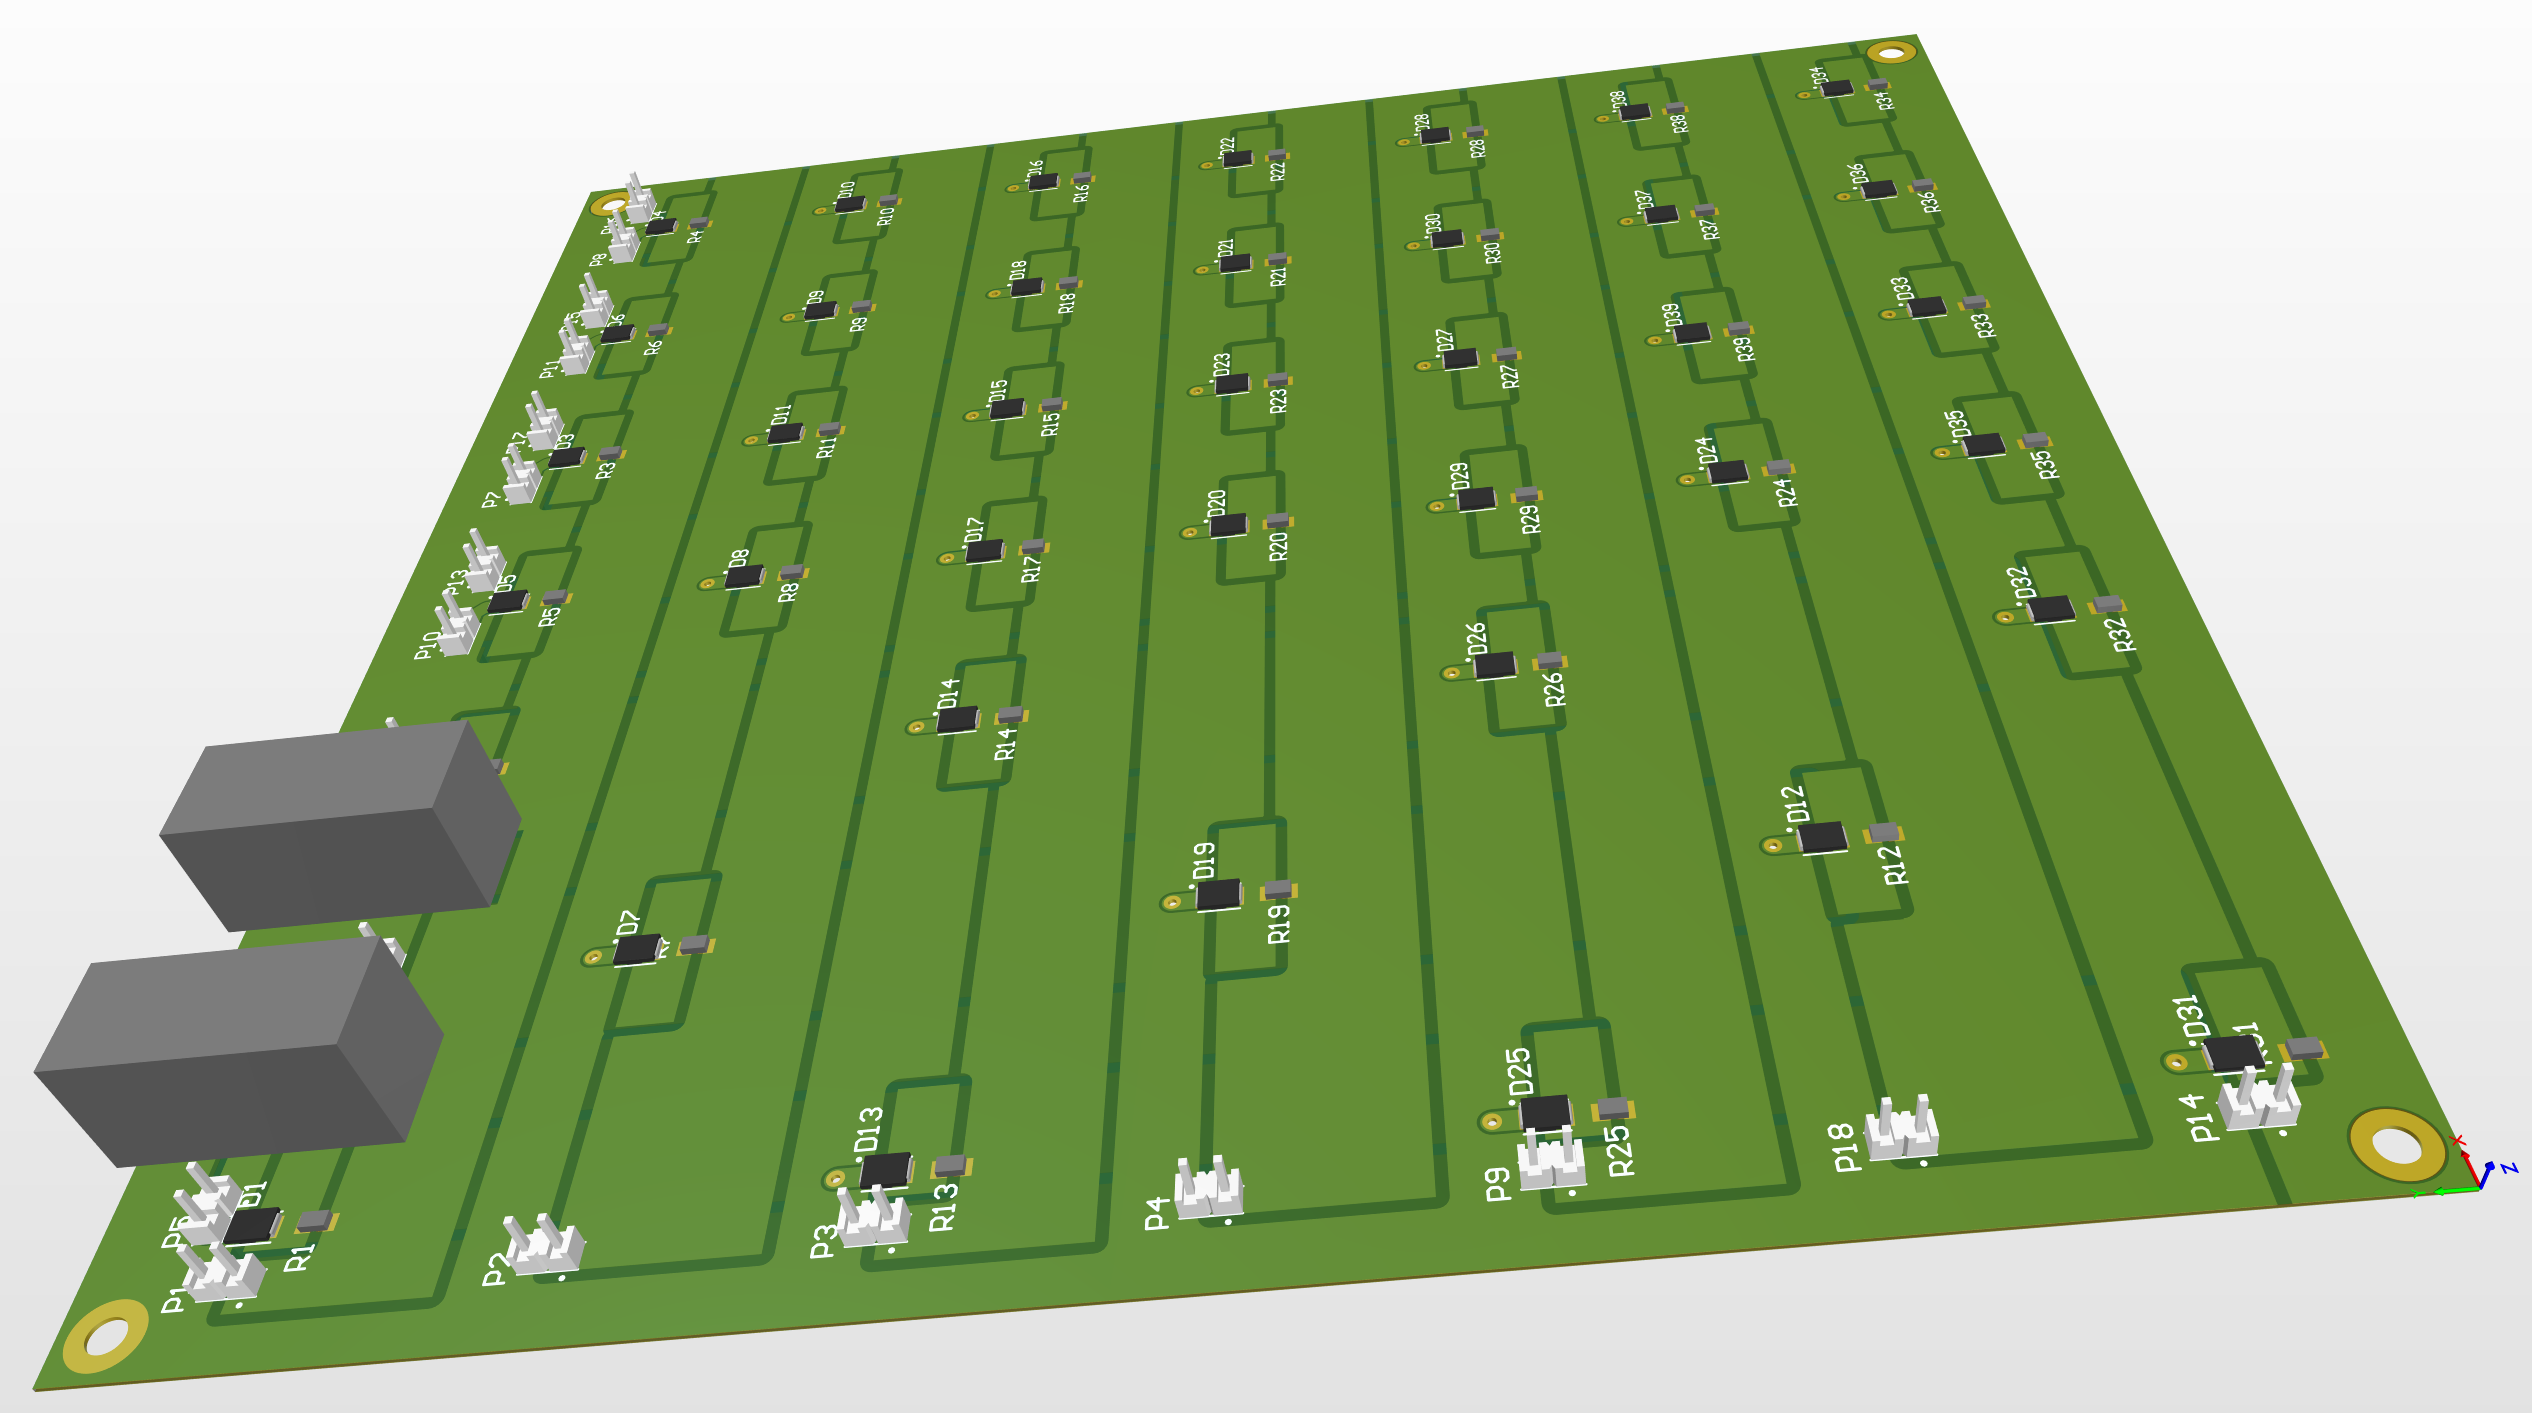
\includegraphics[width=0.9\textwidth]{3-development/images/Backlight.png}
	\caption{3D-Model of the backlight PCB.\label{development:pcb}}
\end{figure} 
The LEDs have been placed less dense in the center, to compensate that the image is generally darker on it's edges.
This is also called vignetting \cite{vignetting}.

To spread the light evenly, a diffusion filter (Kimoto OptSaver 100ST) is mounted in front of the two PCBs.
To inspect the how the luminance of the backlight is captured by the camera, different images of the backlight are plotted as a surface- and contour-plot.
Firstly, the empty surface (diffusion filter but no geometry pattern) is analyzed in Figure \ref{development:3d0}. 
\begin{figure}[ht]
	\centering
	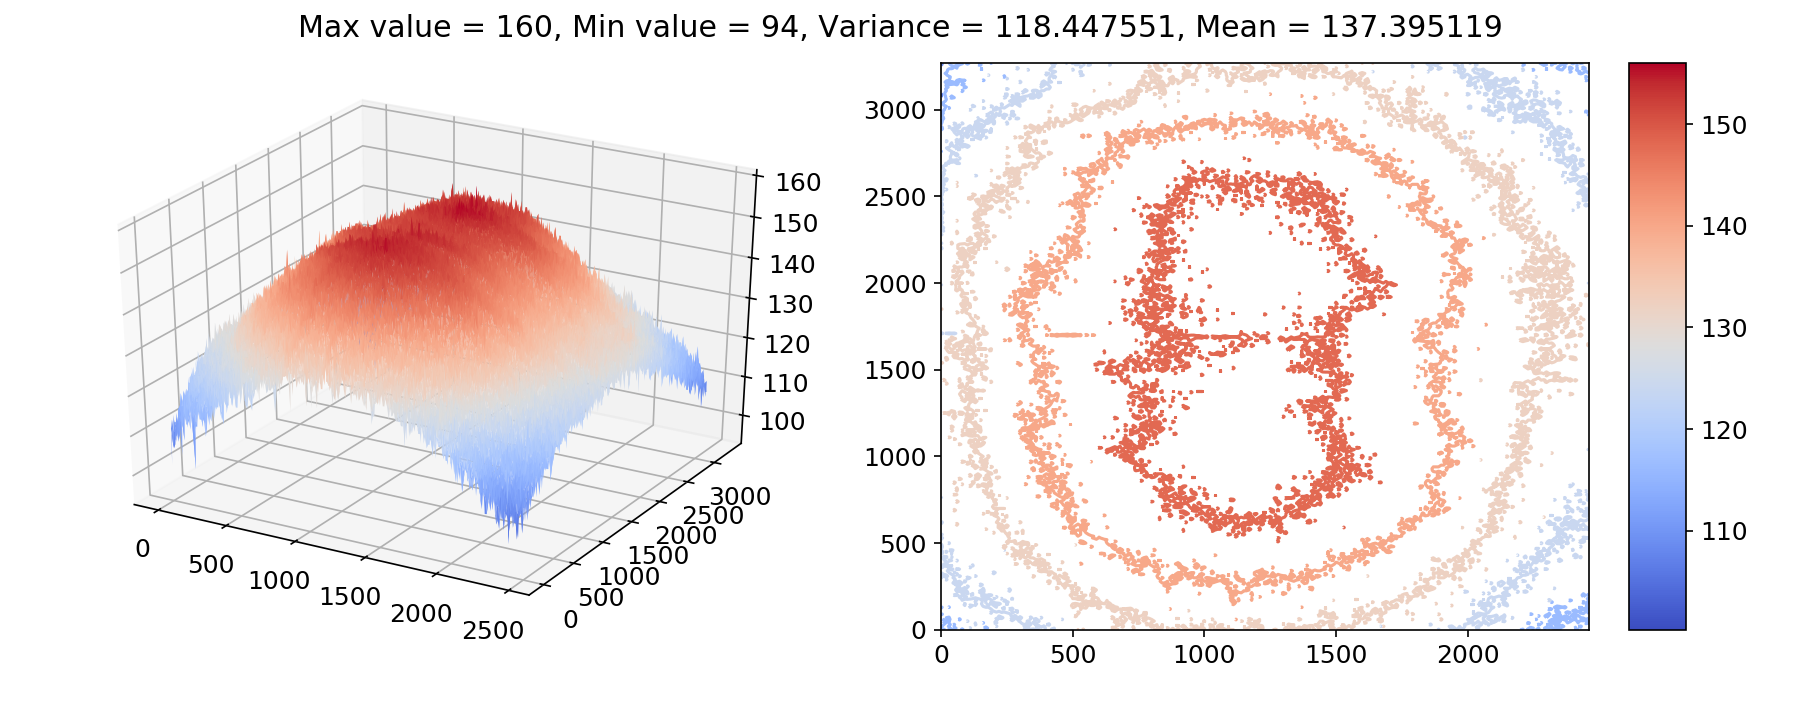
\includegraphics[trim=50 0 0 0,clip,width=0.9\linewidth]{3-development/backlight/3d0.png}
	\caption{Backlight with diffusion filter but no geometry pattern.\label{development:3d0}}
\end{figure} 
In this plot we can spot that our edges are less intense as the middle of our backlight.
With the camera driver regulating our brightness to a mean close to 127, we have a maximum value of 160 and a minimum value of 94.
The image used for the plots in Figure \ref{development:3d1} are taken with the additional geometry pattern on the glass plate.
\begin{figure}[ht]
	\centering
	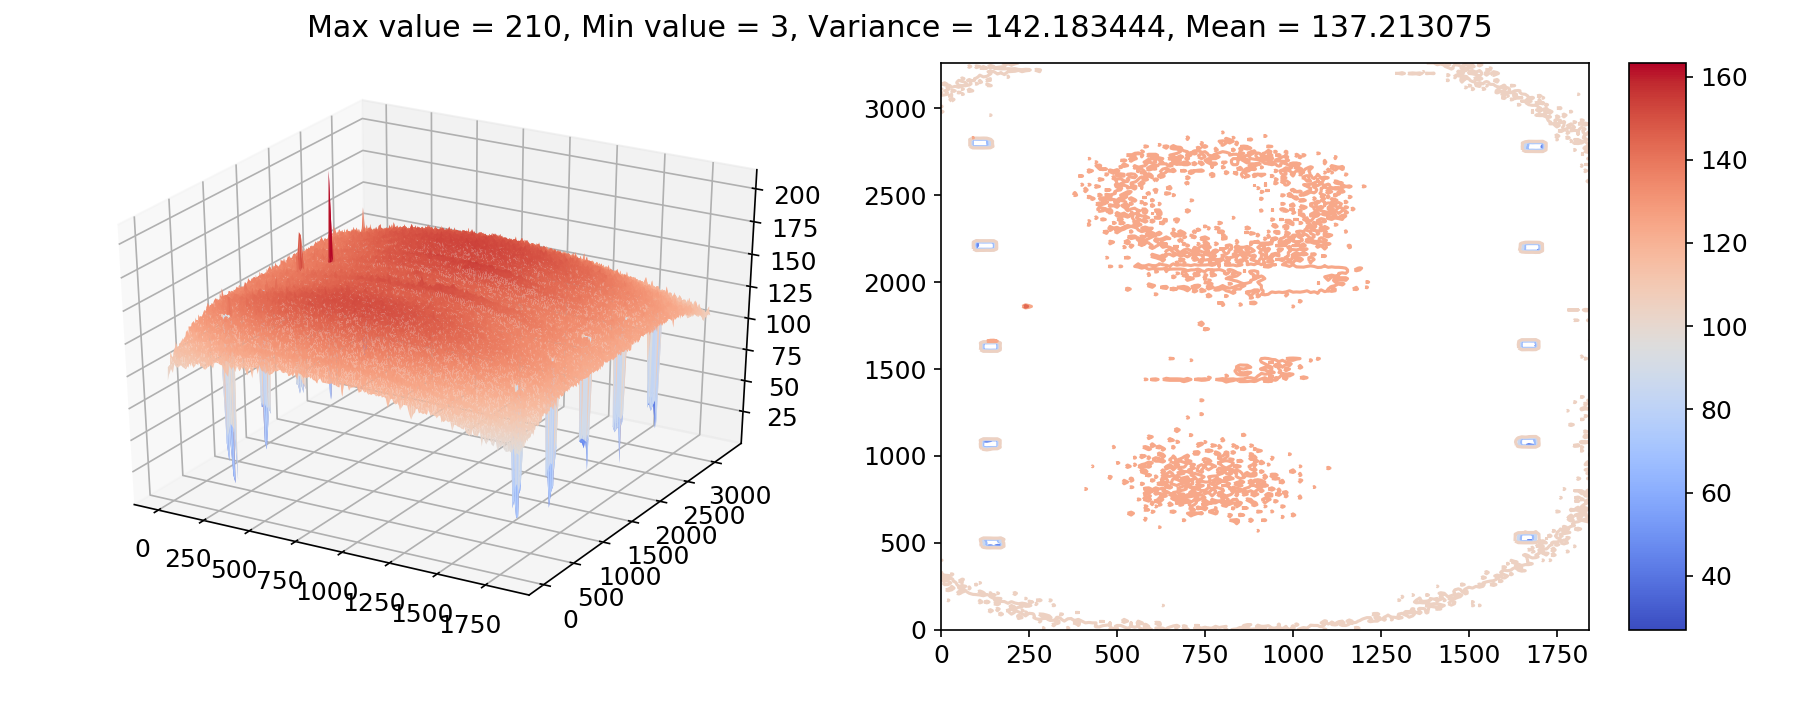
\includegraphics[trim=50 0 0 0,clip,width=0.9\linewidth]{3-development/backlight/3d1.png}
	\caption{Backlight with diffusion filter and geometry pattern.\label{development:3d1}}
\end{figure} 
Now the lowest point lays in the black squares with the value 3.
The maximum value of 210 is an outlier which can be caused by a reflection or not well positioned diffusion filter.
In the plot in Figure \ref{development:3d4} we can see that the some edges of the spring are very close to the background brightness.
\begin{figure}[ht]
	\centering
	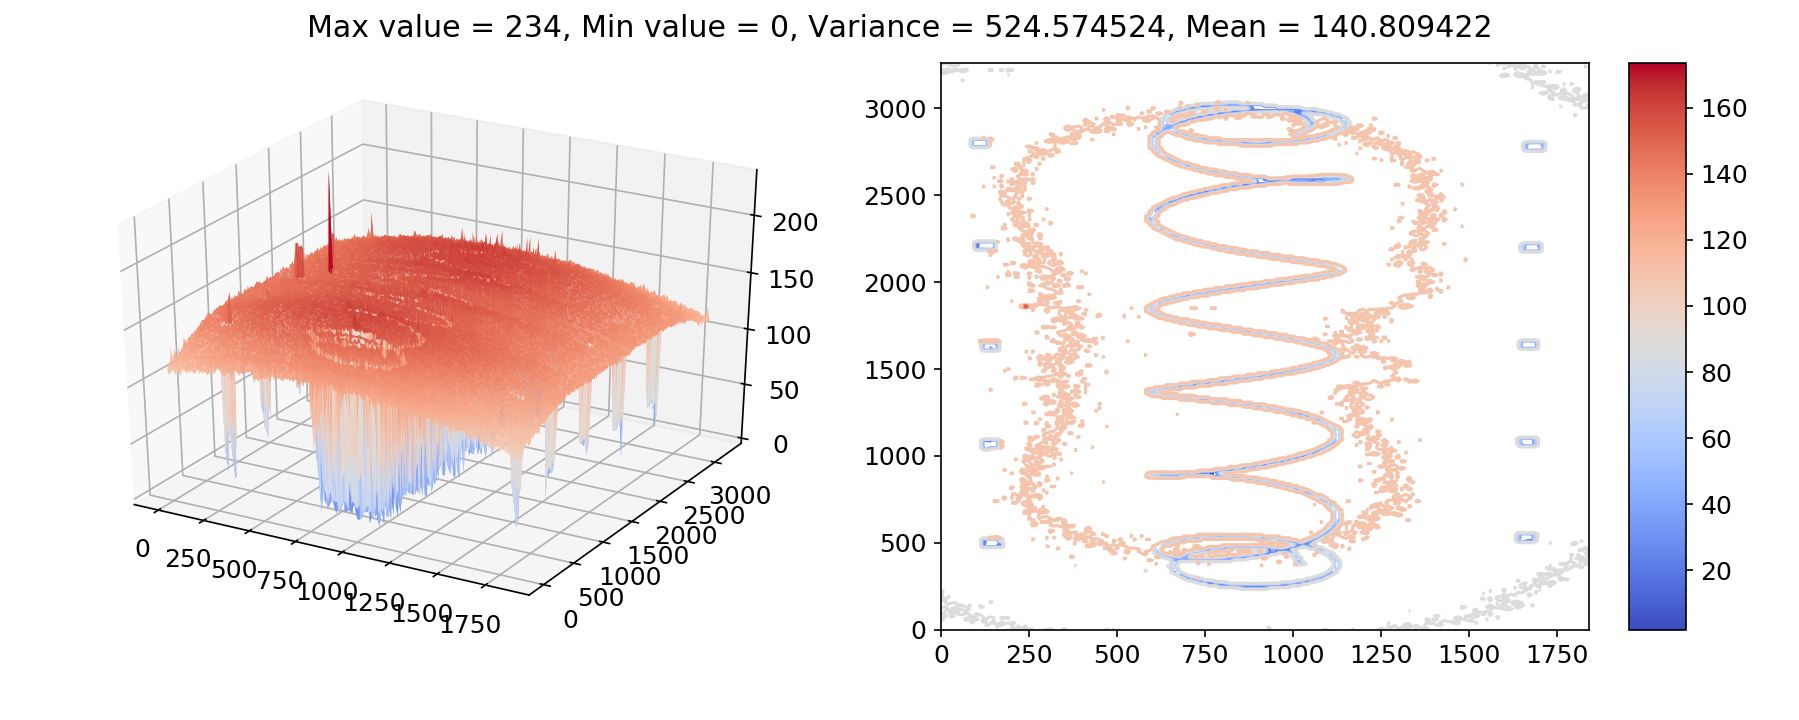
\includegraphics[trim=50 0 0 0,clip,width=0.9\linewidth]{3-development/backlight/3d4.png}
	\caption{Backlight with diffusion filter, geometry pattern and object (spring).\label{development:3d4}}
\end{figure} 
This happens because there is stray light illuminating the edge of the spring.
Since the object is three dimensional, the parts closer to the backlight (on the plane) are illuminated more by stray light than parts further away.

\subsection{Demonstrator}
The demonstrator consists of three essential components.
A mechanical construction made out of aluminum profiles, the backlight with the glass plate and the Jetson Nano with the Raspberry Pi camera.  
This construction as shown in Figure \ref{development:demo} makes it easy to make adjustments in distance and position of the parts, while developing the software.
\begin{figure}[ht]
	\centering
	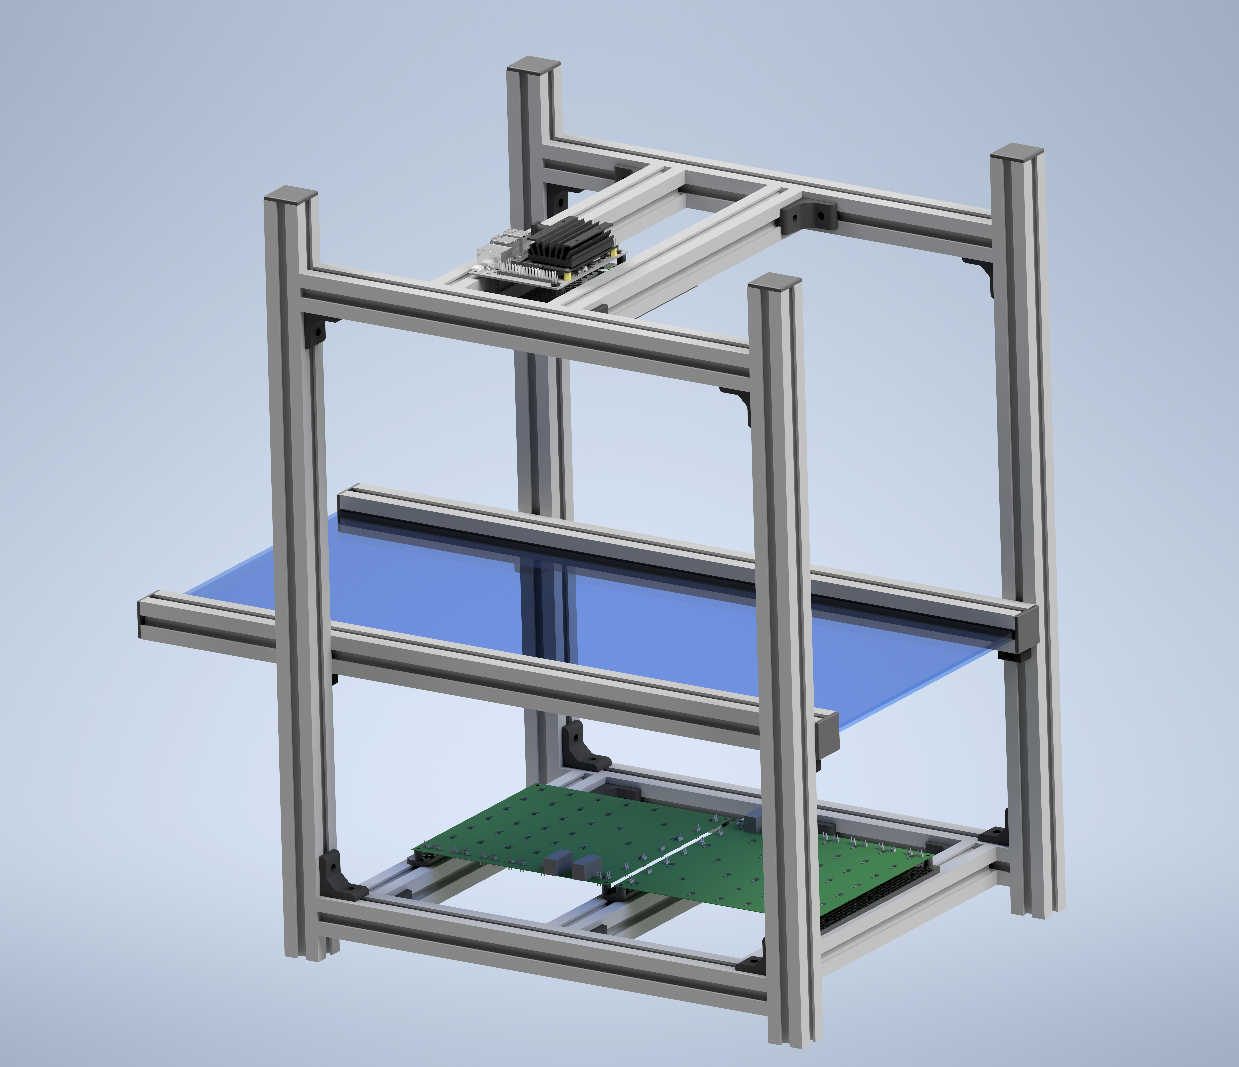
\includegraphics[width=0.9\textwidth]{3-development/images/Demonstrator.png}
	\caption{3D-Model of the demonstrator.\label{development:demo}}
\end{figure} 
The whole construction can be tilted.
This makes it possible to let objects slide through the field of view of the camera, to simulate dynamic measuring.

\subsection{Production cost}
Table \ref{development:cost} lists the cost of the Demonstrator.
Note that the price of one PCB drops to 1.35\,CHF if a batch of 2000 is ordered.
\begin{table}[ht]
	\centering
	\begin{tabular}{|l|c|c|c|}
		\hline
		Component & quantity & price per unit (CHF)& total (CHF)\\
		\hline
		Glass & 3 & 10.95 & 32.85\\
		\hline
		Raspberry Pi camera&1&31.90&31.90\\
		\hline
		Jetson Nano developer kit&1&158.40&158.40\\
		\hline	
		Aluminum profiles and accessories&1&437.40&437.40\\
		\hline
		PCB&2&53.06&106.12\\
		\hline
		LED white 76\,lm&78&0.035&2.73\\
		\hline
		Resistor 13\,$\Omega$&78&0.043&3.354\\
		\hline
		Jumper&36&0.037&1.332\\
		\hline
		Socket&4&2.02&8.08\\
		\hline
		\hline
		\textbf{Total}&&&728.168\\
		\hline
	\end{tabular}
	\caption{Demonstrator costs.\label{development:cost}}
\end{table}
\newpage
\section{Backlight}
To goal of having a cheap demonstrator is fully depended on the hardware cost since software is always free to distribute. With this goal in mind we developed a cheap backlight which consists of a fixed PCB panel and a diffusion filter mounted in front of the LED's to spread the light evenly. 

\section{Camera Calibration in OpenCV\label{theory:calibration}}
A camera has to be calibrated in order to obtain camera parameters like focal length and center-point.
Further, it provides a method to correct distortions caused by the imperfect optics according to a certain distortion model.
For that, images of a known pattern (usually a checkerboard) have to be taken from different view-points an angles.
These points provide the training data which is needed to estimate all the coefficients.

This section describes the theory behind the calibration process in OpenCV.
The subsections \ref{theory:pinhole} and \ref{theory:distortion} adapt parts of theory and notation from the OpenCV 4.3.0 documentation \cite{cv_calib}, which is the latest version at the time of writing this thesis.

\subsection{The pinhole camera model\label{theory:pinhole}}
The functions OpenCV provides to calibrate the camera use the so-called pinhole camera model.
This model describes, how a 3D-point specified in world-coordinates ($P_w$) is transformed to a 3D-point in camera-coordinates ($P_c$) and then further projected onto the image plane ($p$). After this step, the point is described as a 2D-point in pixel coordinates. The pinhole-model is shown in Figure \ref{theory:pin1}.
\begin{figure}[ht]
	\centering
	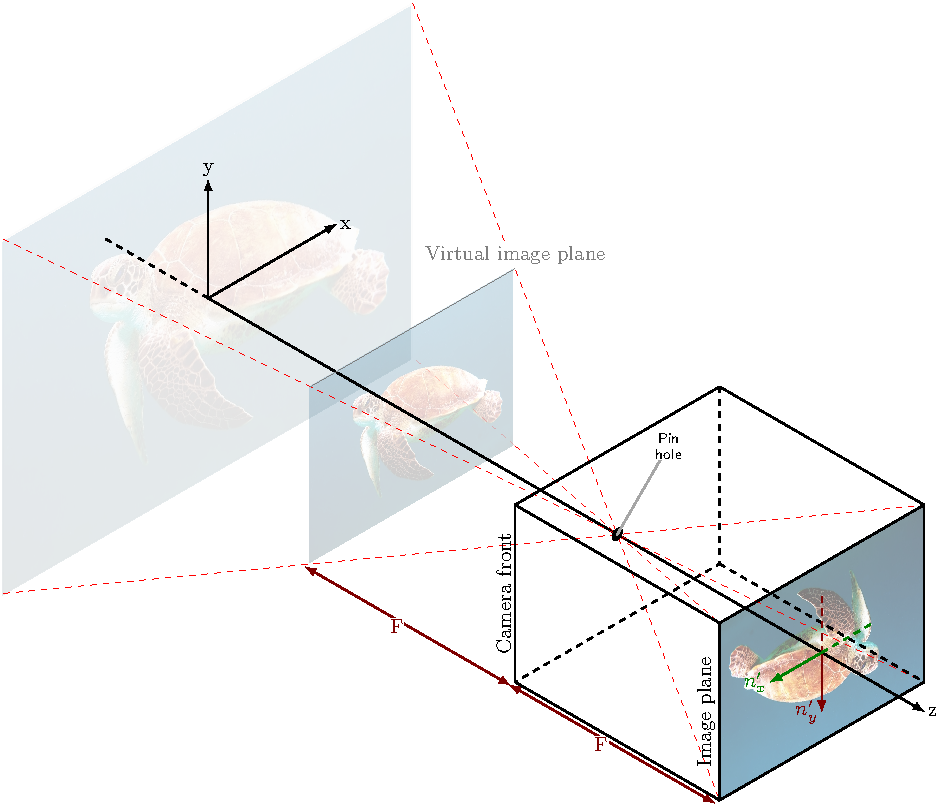
\includegraphics[width=0.9\textwidth]{2-theory/cam/Camera2.pdf}
	\caption{The pinhole camera model.\label{theory:pin1}}
\end{figure} 
This setup is simplified by mirroring the image plane at the pinhole, as shown in Figure \ref{theory:pin2}.
\begin{figure}[ht]
	\centering

	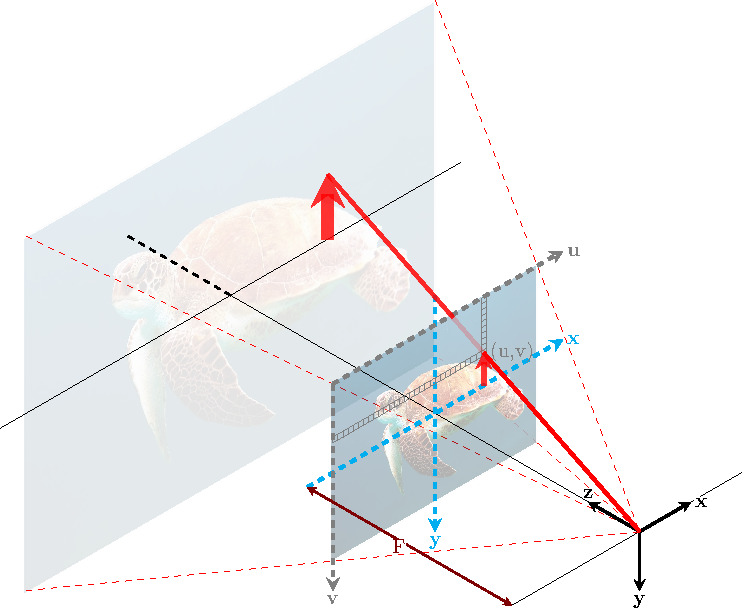
\includegraphics[width=0.9\textwidth]{2-theory/cam/camera3.pdf}
	\caption{The simplified camera model.\label{theory:pin2}}
\end{figure}

The transition from the world-coordinates to the camera-coordinates can be described as 
\begin{align*}
\underbrace{\begin{pmatrix}
X_c\\
Y_c\\
Z_c\\
\end{pmatrix}}_{P_c}=
\underbrace{\begin{pmatrix}
r_{11}&r_{12}&r_{13}\\
r_{21}&r_{22}&r_{23}\\
r_{31}&r_{32}&r_{33}
\end{pmatrix}}_{R}
\underbrace{\begin{pmatrix}
X_w\\
Y_w\\
Z_w\\
\end{pmatrix}}_{P_w}+
\underbrace{\begin{pmatrix}
t_x\\
t_y\\
t_z\\
\end{pmatrix}}_{t}.
\end{align*}
The vector $P_w$ is first rotated by $R$ and the translated by $t$. This can be written as one single matrix:
\begin{align}
\begin{pmatrix}
X_c\\
Y_c\\
Z_c
\end{pmatrix}=
\begin{pmatrix}
r_{11}&r_{12}&r_{13}&t_x\\
r_{21}&r_{22}&r_{23}&t_y\\
r_{31}&r_{32}&r_{33}&t_z
\end{pmatrix}
\begin{pmatrix}
X_w\\
Y_w\\
Z_w\\
1
\end{pmatrix}\quad\Leftrightarrow\quad
P_c=
\begin{pmatrix}
R&|&t
\end{pmatrix}
\begin{pmatrix}
P_w\\
1
\end{pmatrix}\label{theory:world-camera}.
\end{align}

As a result of the theorem of intersecting lines, the projection from $P_c$ to $p$ is described as
\begin{align*}
\underbrace{\begin{pmatrix}
u\\
v
\end{pmatrix}}_{p}=
\begin{pmatrix}
f_x\cdot X_c/Z_c\\
f_y\cdot Y_c/Z_c\\
\end{pmatrix}+
\begin{pmatrix}
c_x\\
c_y
\end{pmatrix}.
\end{align*}
where $f_x$ and $f_y$ are the focal length $F$ (in world units) normalized by their respective pixel size (in world units). Thus $f_x$ and $f_y$ are the same, if the pixels are quadratic.

By adding the principal point $(c_x\quad c_y)^T$, which is usually close to the image center, it is taken into account, that the origin of the pixel-coordinates is placed in the upper left corner of the image plane.
It is now simpler to write this in homogeneous coordinates:
\begin{align}
\begin{pmatrix}
u\\
v\\
1
\end{pmatrix}\sim s
\begin{pmatrix}
u\\
v\\
1
\end{pmatrix}=
\underbrace{\begin{pmatrix}
f_x&0&c_x\\
0&f_y&c_y\\
0&0&1
\end{pmatrix}}_{K}
\begin{pmatrix}
X_c\\
Y_c\\
Z_c
\end{pmatrix}\quad \Leftrightarrow \quad s
\begin{pmatrix}
p\\
1
\end{pmatrix}=
K\cdot P_c
\label{theory:camera-pixel},
\end{align}
where $s$ is an arbitrary scaling factor and $K$ is called the camera matrix.
The overall transition from world- to pixel-coordinates is the result of combining \ref{theory:world-camera} and \ref{theory:camera-pixel}:
\begin{align}
s
\begin{pmatrix}
u\\
v\\
1
\end{pmatrix}=
\begin{pmatrix}
f_x&0&c_x\\
0&f_y&c_y\\
0&0&1
\end{pmatrix}
\begin{pmatrix}
r_{11}&r_{12}&r_{13}&t_x\\
r_{21}&r_{22}&r_{23}&t_y\\
r_{31}&r_{32}&r_{33}&t_z
\end{pmatrix}
\begin{pmatrix}
X_w\\
Y_w\\
Z_w\\
1
\end{pmatrix}\quad \Leftrightarrow \quad s
\begin{pmatrix}
p\\
1
\end{pmatrix}=
K
\begin{pmatrix}
R&|&t
\end{pmatrix}
\begin{pmatrix}
P_w\\
1
\end{pmatrix}\label{theory:world-pixel}
\end{align}
The rotation and translation in $\begin{pmatrix}R&|&t\end{pmatrix}$ are called the extrinsic parameters. The camera matrix $K$ contains analogously the linear intrinsic parameters.

\subsection{The distortion model in OpenCV\label{theory:distortion}}
Non linear distortions, which appear before the projection in \ref{theory:camera-pixel} should be considered too.
OpenCV compensates the effects of radial, tangential and thin prism distortion.
\subsubsection{Radial Distortion}
Radial distortion is caused by the flawed curvature of the lens \cite{weng}.
It can be modeled with
\begin{align}
\begin{pmatrix}
x''\\
y''
\end{pmatrix}=
\begin{pmatrix}
x'\frac{1+k_1 r^2+k_2 r^4+k_3 r^6}{1+k_4 r^2+k_5r^4+k_6r^6}\\
y'\frac{1+k_1 r^2+k_2 r^4+k_3 r^6}{1+k_4 r^2+k_5r^4+k_6r^6}
\end{pmatrix}\label{theory:raddist},
\end{align}
where $x'$ and $y'$ are coordinates, described in camera-coordinates, normalized with $Z_c$
\begin{align*}
\begin{pmatrix}
x'\\
y'
\end{pmatrix}=
\begin{pmatrix}
X_c/Z_c\\
Y_c/Z_c
\end{pmatrix}
\end{align*}
and r is the radius as taken with respect to the principal point $(c_x\quad c_y)^T$
\begin{align*}
r^2 = x'^2 + y'^2.
\end{align*}
This type of distortion is symmetrical with respect to the principal point.
Figure \ref{theory:radial} illustrates the effect on a rectangle.
\begin{figure}[ht]
	\centering
	\includegraphics[width=0.9\textwidth]{2-theory/calibration/distortion/radial.png}
	\caption{Different types of radial distortion. Black: no distortion, red: $k_1 = 10$, $k_2=11$, $k_3=12$, $k_4=5$, $k_5=6$, $k_6=7$, blue: $k_1 = -2.2$, $k_2=-1.2$, $k_3=-0.8$, $k_4=-0.4$, $k_5=-0.3$, $k_6=-0.2$.\label{theory:radial}}
\end{figure} 

\subsubsection{Tangential distortion}
Real optical systems are also modified by the effects of tangential distortion. This type of distortion has a decentering effect and occurs, if the line through the optical center of the lens and the principal point is not col-linear with the optical axis \cite{weng}.
The model
\begin{align}
\begin{pmatrix}
x''\\
y''
\end{pmatrix}=
\begin{pmatrix}
x' + 2p_1x'y'+p_2(r^2+2x'^2)\\
y' + 2p_2x'y'+p_1(r^2+2y'^2)
\end{pmatrix}\label{theory:tandist}
\end{align}
takes this into account.
Figure \ref{theory:tangential} shows the distortion this model introduces.

\begin{figure}[ht]
	\centering
	\includegraphics[width=0.9\textwidth]{2-theory/calibration/distortion/tangential.png}
	\caption{Different types of tangential distortion (example adapted from \cite{weng}), black: no distortion, red: $p_1 = -0.15$, $p_2=-0.4$, blue: $p_1 = 0.15$, $p2=-0.4$.\label{theory:tangential}}
\end{figure} 

\subsubsection{Thin prism distortion}
Thin prism distortion is partially caused by lens imperfections and camera assembly \cite{weng}.
It introduces additional radial and tangential distortion, modeled with
\begin{align}
\begin{pmatrix}
x''\\
y''
\end{pmatrix}=
\begin{pmatrix}
x' + s_1 r^2 + s_2 r^4\\
y' + s_3 r^2 + s_4 r^4
\end{pmatrix}\label{theory:prismdist}.
\end{align}

\subsubsection{The combined model in OpenCV}
The models in \ref{theory:raddist}, \ref{theory:tandist} and \ref{theory:prismdist} combined result in
\begin{align}
\begin{pmatrix}
x''\\
y''
\end{pmatrix}=
\begin{pmatrix}
x'\frac{1+k_1 r^2+k_2 r^4+k_3 r^6}{1+k_4 r^2+k_5r^4+k_6r^6}+2p_1 x' y'+p_2(r^2+2x'^2)+s_1 r^2+s_2 r^4\\
y'\frac{1+k_1 r^2+k_2 r^4+k_3 r^6}{1+k_4 r^2+k_5r^4+k_6r^6}+2p_2x'y'+p_1(r^2+2y'^2)+s_3 r^2+s_4 r^4
\end{pmatrix}\label{theory:dist}.
\end{align}
In summary, a point in normalized camera-coordinates $(x'\quad y')^T$ is distorted as modeled in \ref{theory:dist}, which leads to the point $(x'' \quad y'')^T$. To get the distorted pixel-coordinates (index $d$), the projection has to be applied
\begin{align*}
\begin{pmatrix}
u_d\\
v_d\\
\end{pmatrix}=
\begin{pmatrix}
x''f_x+c_x\\
y''f_y+c_y
\end{pmatrix}\quad\Leftrightarrow\quad
\begin{pmatrix}
u_d\\
v_d\\
1
\end{pmatrix}=K
\begin{pmatrix}
x''\\
y''\\
1
\end{pmatrix},
\end{align*}
which completes the model so far.
Keep in mind, that when correcting the distortion, equation \ref{theory:dist} has to be inverted.

\subsection{Reprojection error}
The reprojection error is a value to assess the quality of a calibration.
It is the error between the detected image point and the projection (using the obtained coefficients) of its corresponding world point onto the image plane.
Since it only uses the points, which where previously used to obtain the calibration-parameters, it can be interpreted as a training error rate.

Calibration functions in OpenCV return the overall \acs{rms} reprojection error \cite{cv_calib}.

\subsection{Error propagation as further quality assessment\label{theory:error_propagation}}
As argued before, the reprojection error is a training error rate.
A low reprojection error is therefore not necessarily enough to estimate, how good the calibration really performs.

OpenCV returns with its extended calibration functions not only the camera intrinsics, but also an estimated standard deviation of each coefficient \cite{cv_calib}.
Under assumption that low standard deviations suggest a good calibration, it is valid to combine all standard deviations into one value, using the propagation of uncertainty.

The propagation of error (theory taken from \cite{benno}) states that influence of each error of the inputs $x_i$ on the output value $y$ of a function
\begin{align*}
	y = f(x_1, x_2,...,x_n)
\end{align*}
can be linearly approximated and summed up to:
\begin{align}
	\Delta y = \sqrt{\sum_{i=1}^{n}\left(\frac{\partial y}{\partial x_i}\Delta x_i \right)^2} \label{theory:prop}.
\end{align}

Applied to \ref{theory:dist}, this leads to
\begin{align*}
	\Delta x''=\sqrt{\sum_{i=1}^{6}\left(\frac{\partial x''}{\partial k_i}\Delta k_i \right)^2+\sum_{i=1}^{2}\left( \frac{\partial x''}{\partial p_i}\Delta p_i\right)^2+\sum_{i=1}^{4}\left( \frac{\partial x''}{\partial s_i}\Delta s_i\right)^2}
\end{align*}
and
\begin{align*}
	\Delta y''=\sqrt{\sum_{i=1}^{6}\left(\frac{\partial y''}{\partial k_i}\Delta k_i \right)^2+\sum_{i=1}^{2}\left( \frac{\partial y''}{\partial p_i}\Delta p_i\right)^2+\sum_{i=1}^{4}\left( \frac{\partial y''}{\partial s_i}\Delta s_i\right)^2}.
\end{align*}
The computed derivatives are listed in the appendix.
If we look at pixel coordinates with respect to the center of the image, the radius (distance from the center-point) can be expressed as
\begin{align*}
	r = \sqrt{(f_x\cdot x'')^2+(f_y\cdot y'')^2}
\end{align*}
and therefore, if errors in $f_x$ and $f_y$ are neglected, with the propagation in \ref{theory:prop} applied
\begin{align}
	\Delta r = \sqrt{\left(\frac{\partial r}{\partial x''} \Delta x''\right)^2+\left(\frac{\partial r}{\partial y''} \Delta y''\right)^2}\label{theory:delta_r}.
\end{align}
The value $\Delta r$ can now be used to compare calibration coefficients of different calibration approaches.

\newpage
\section{Threshold and edge detection}
To measure a object bypassing the camera field the outlines of the object are needed. The challenge here is to find the edges of an object with little computing power in such a short time that the measurement time does not become useless. For further processing the edges have to be represented by an one pixel thick line. This section shows the used method and implementation of the further used edge detection. The ISP driver of the Jetson Nano is used in the automatic mode. In this configuration the ISP tries to keep the mean of the image close to the value 128, which resembles the middle of its range. Since the gStreamer pipeline handling over Python is somewhat complicated, the camera is only used in automatic mode.

\subsection{Threshold}
To determine a good threshold method a short look at the histogram is the first step to success. With a back light it can be expected to have a clear difference between foreground and background of the image. 
\begin{figure}[H]
	\subfigure[\label{development:thre1}]{\fbox{
\includegraphics[width=0.5\linewidth, height=5cm]{3-development/threshold/im0.png}}}
	\subfigure[\label{development:thre2}]{\fbox{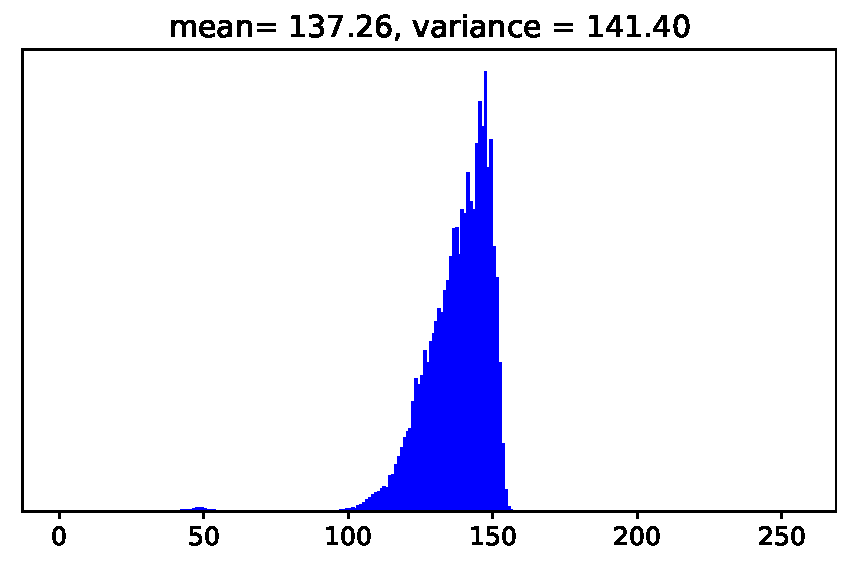
\includegraphics[width=0.5\linewidth, height=5cm]{3-development/threshold/hist_pattern2.pdf}}}
	\subfigure[\label{development:thre3}]{\fbox{
\includegraphics[width=0.5\linewidth, height=5cm]{3-development/threshold/im1.png}}}
	\subfigure[\label{development:thre4}]{\fbox{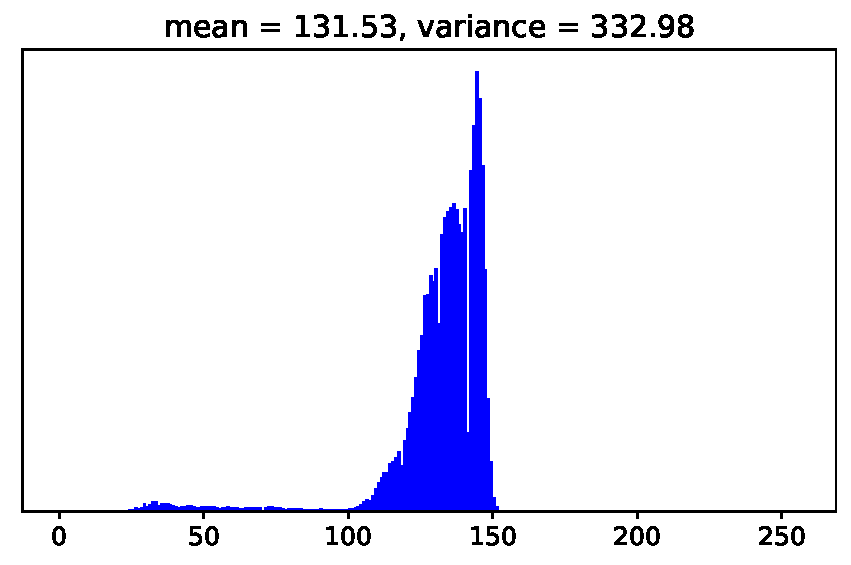
\includegraphics[width=0.5\linewidth, height=5cm]{3-development/threshold/hist_feder2.pdf}}}
	\caption{Histogram of the reference pattern and a spring with running back light\label{development:thre}}	
\end{figure}
\newpage
In the picture \ref{development:thre1} the back light is running and the calibration pattern is in place but no object to measure. The corresponding histogram \ref{development:thre2} shows that nearly every pixel belongs to the background white which is between the value 100 and 155. If a object enters the field of view of the camera it is displayed as black and we get more small values. This shift is also reproduced by the variance. The mean itself is getting corrected by the ISP and can not be used to detect if an object is in the image or not.\\
The obvious answer for a threshold would now be to just cut the histogram around the value 100 in two and set the values to black and white. But with the automatic ISP there is a good chance to loose important information if there is no adaptive threshold. Since the goal is to get as much information as possible from the edges, a little bit of noise can be handled. The method which produced the best results with a back light, was the triangle method \ref{theory:triangle}.

The triangle method calculates the value 112 on the given image \ref{development:thre3} which, using a binary threshold, results in the image \ref{development:thresh}. It is visible that we get a lot of noise in the edges of the resulting picture. \\
\begin{center}
	%\centering
	\fbox{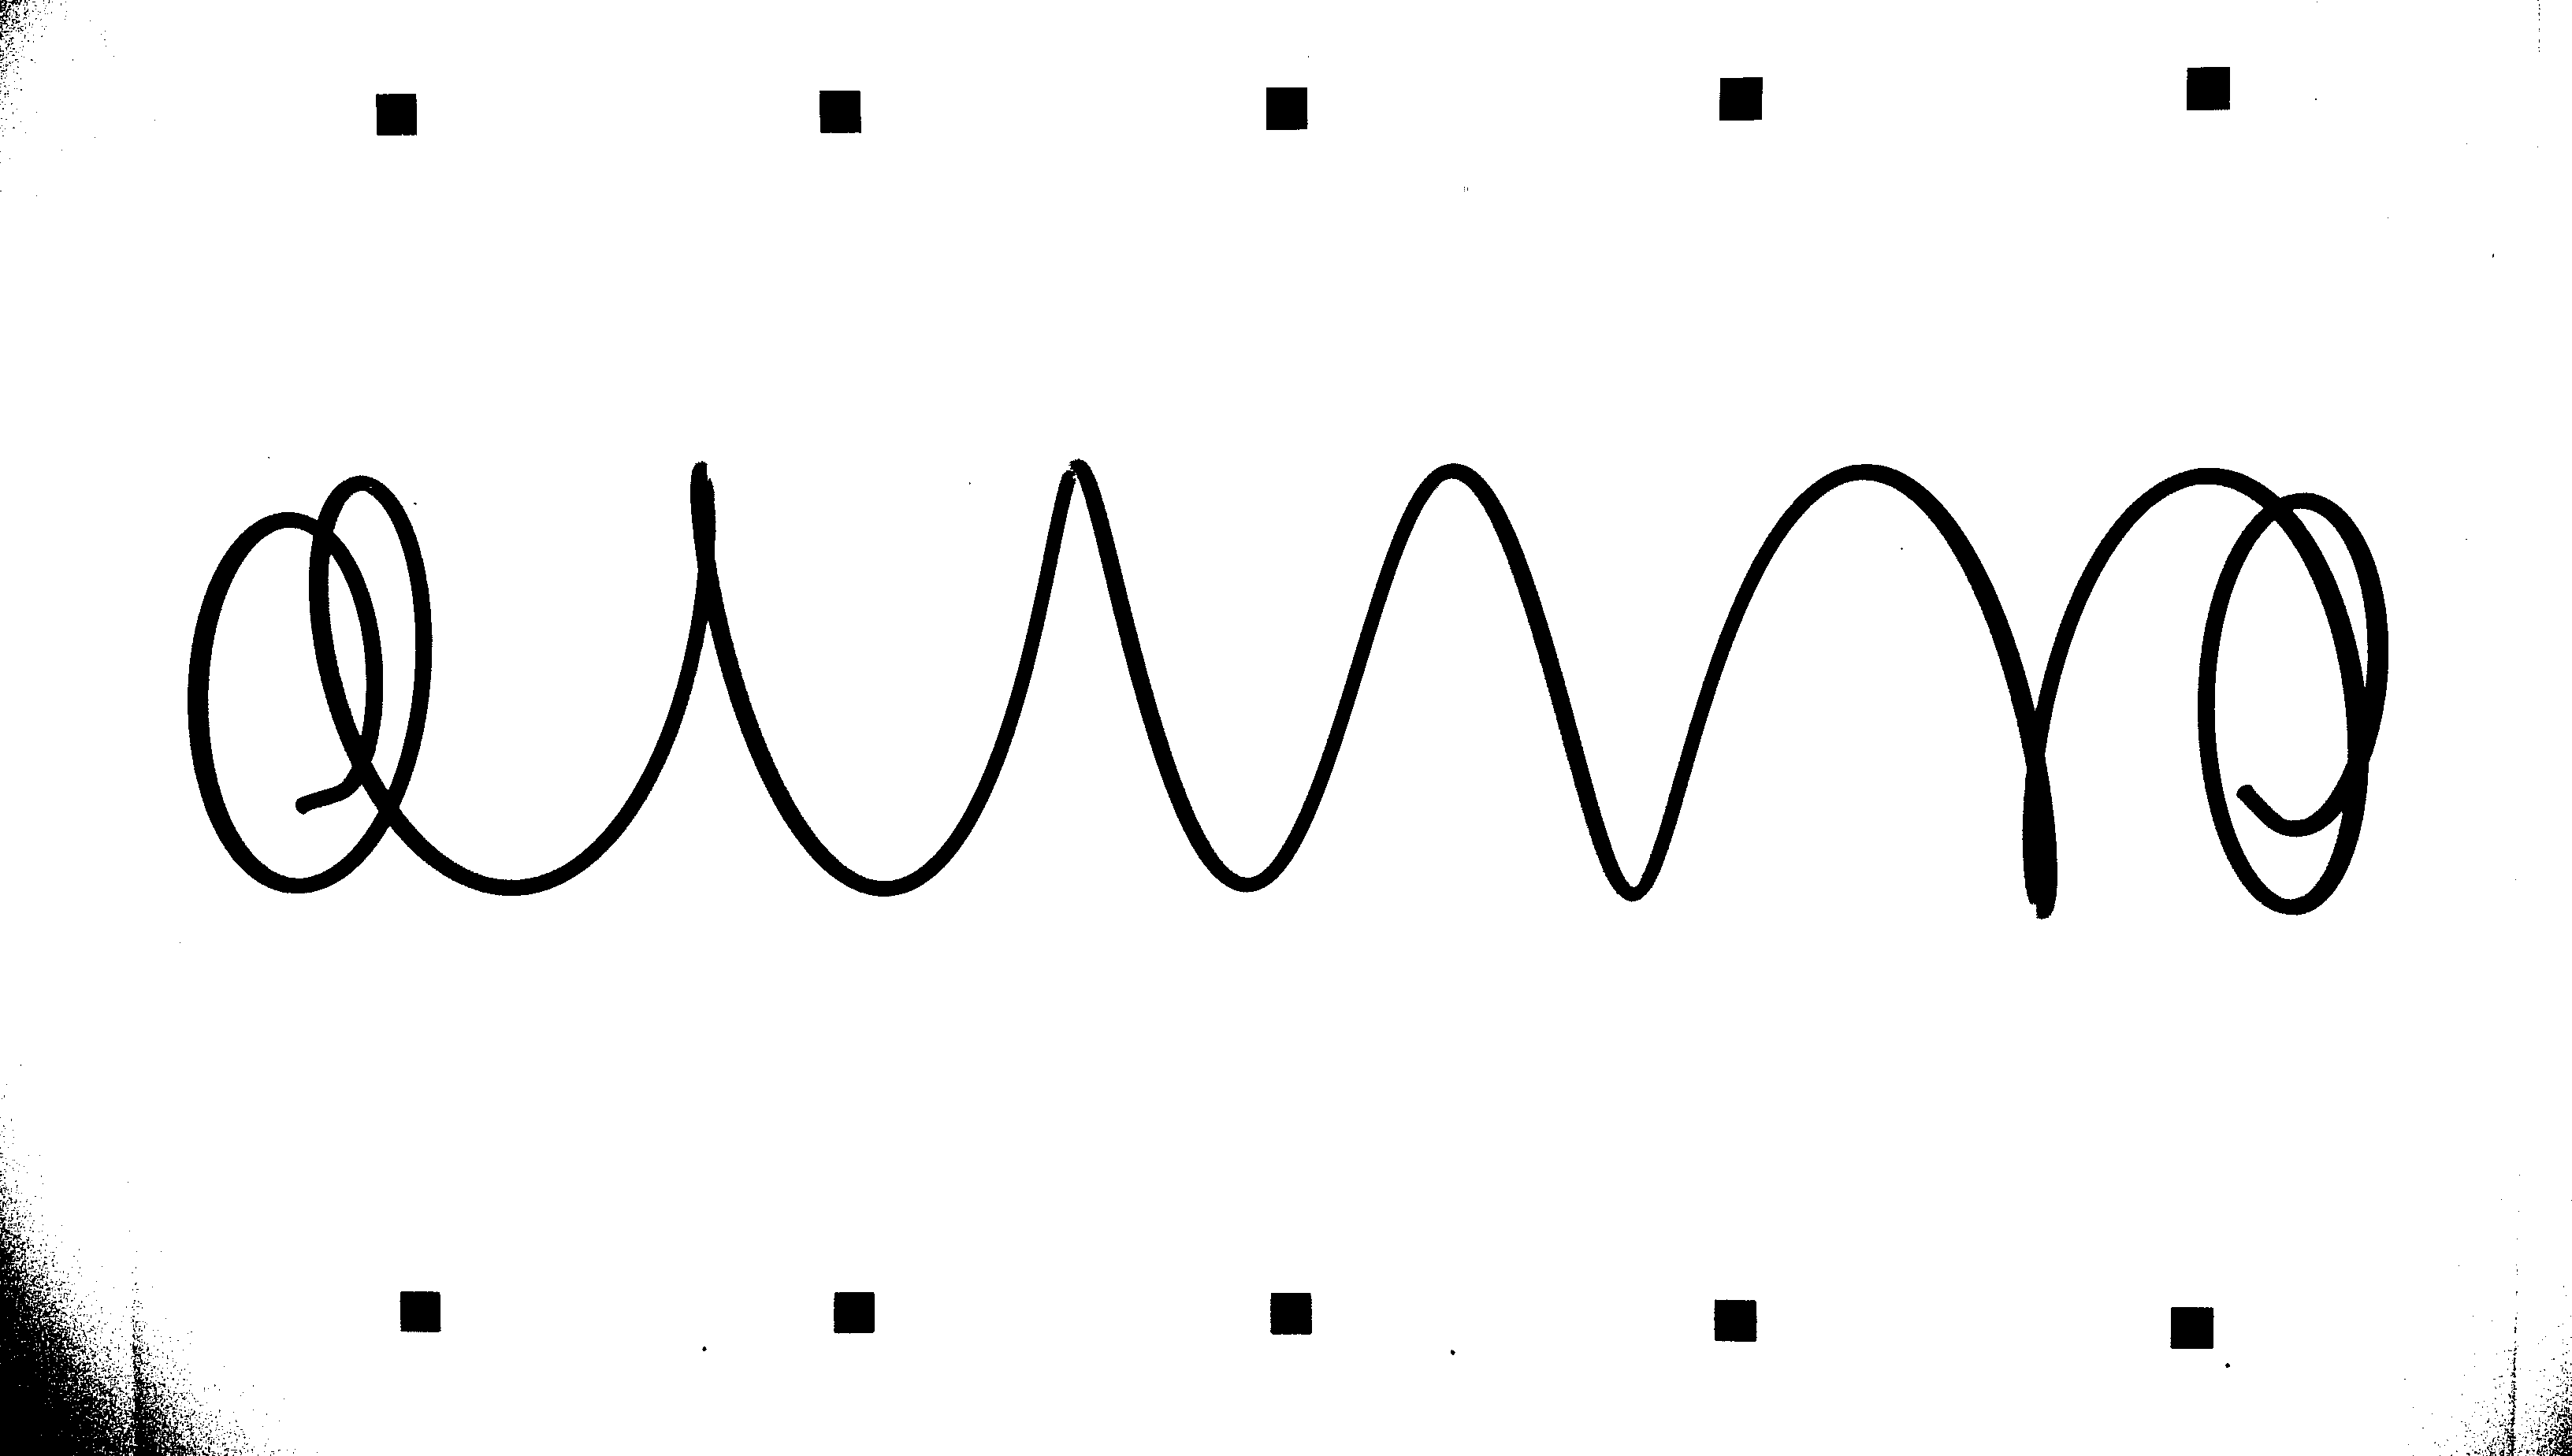
\includegraphics[width=0.9\linewidth]{3-development/threshold/threshold.png}}
	\captionof{figure}{Image after triangle threshold with threshold value 112}
	\label{development:thresh}
\end{center}
since the noise occurs only in the edges of the image it can dealt with ease. The focus lies more on the pattern and spring which should lose as few information as possible.

Another very popular method for an global adaptive threshold is the otsu algorithm. Otsu's goal is to maximize the variance of the fore and background in a image as good as possible in the histogram. Also known as the between-class variance. The result of an otsu threshold on the given image \ref{development:thre3} can be seen in the image \ref{development:otsu}. On the first sight it looks pretty clean and no noise is visible. Which leads to think that the otsu should be a good algorithm for this problem. But if the images \ref{development:triangle} and \ref{development:otsu} are investigated a little bit closer and compared directly it shows some disadvantage of the otsu which can not be corrected afterwards.\\


\begin{figure}[!h]
	\subfigure[\label{development:triangle}]{\fbox{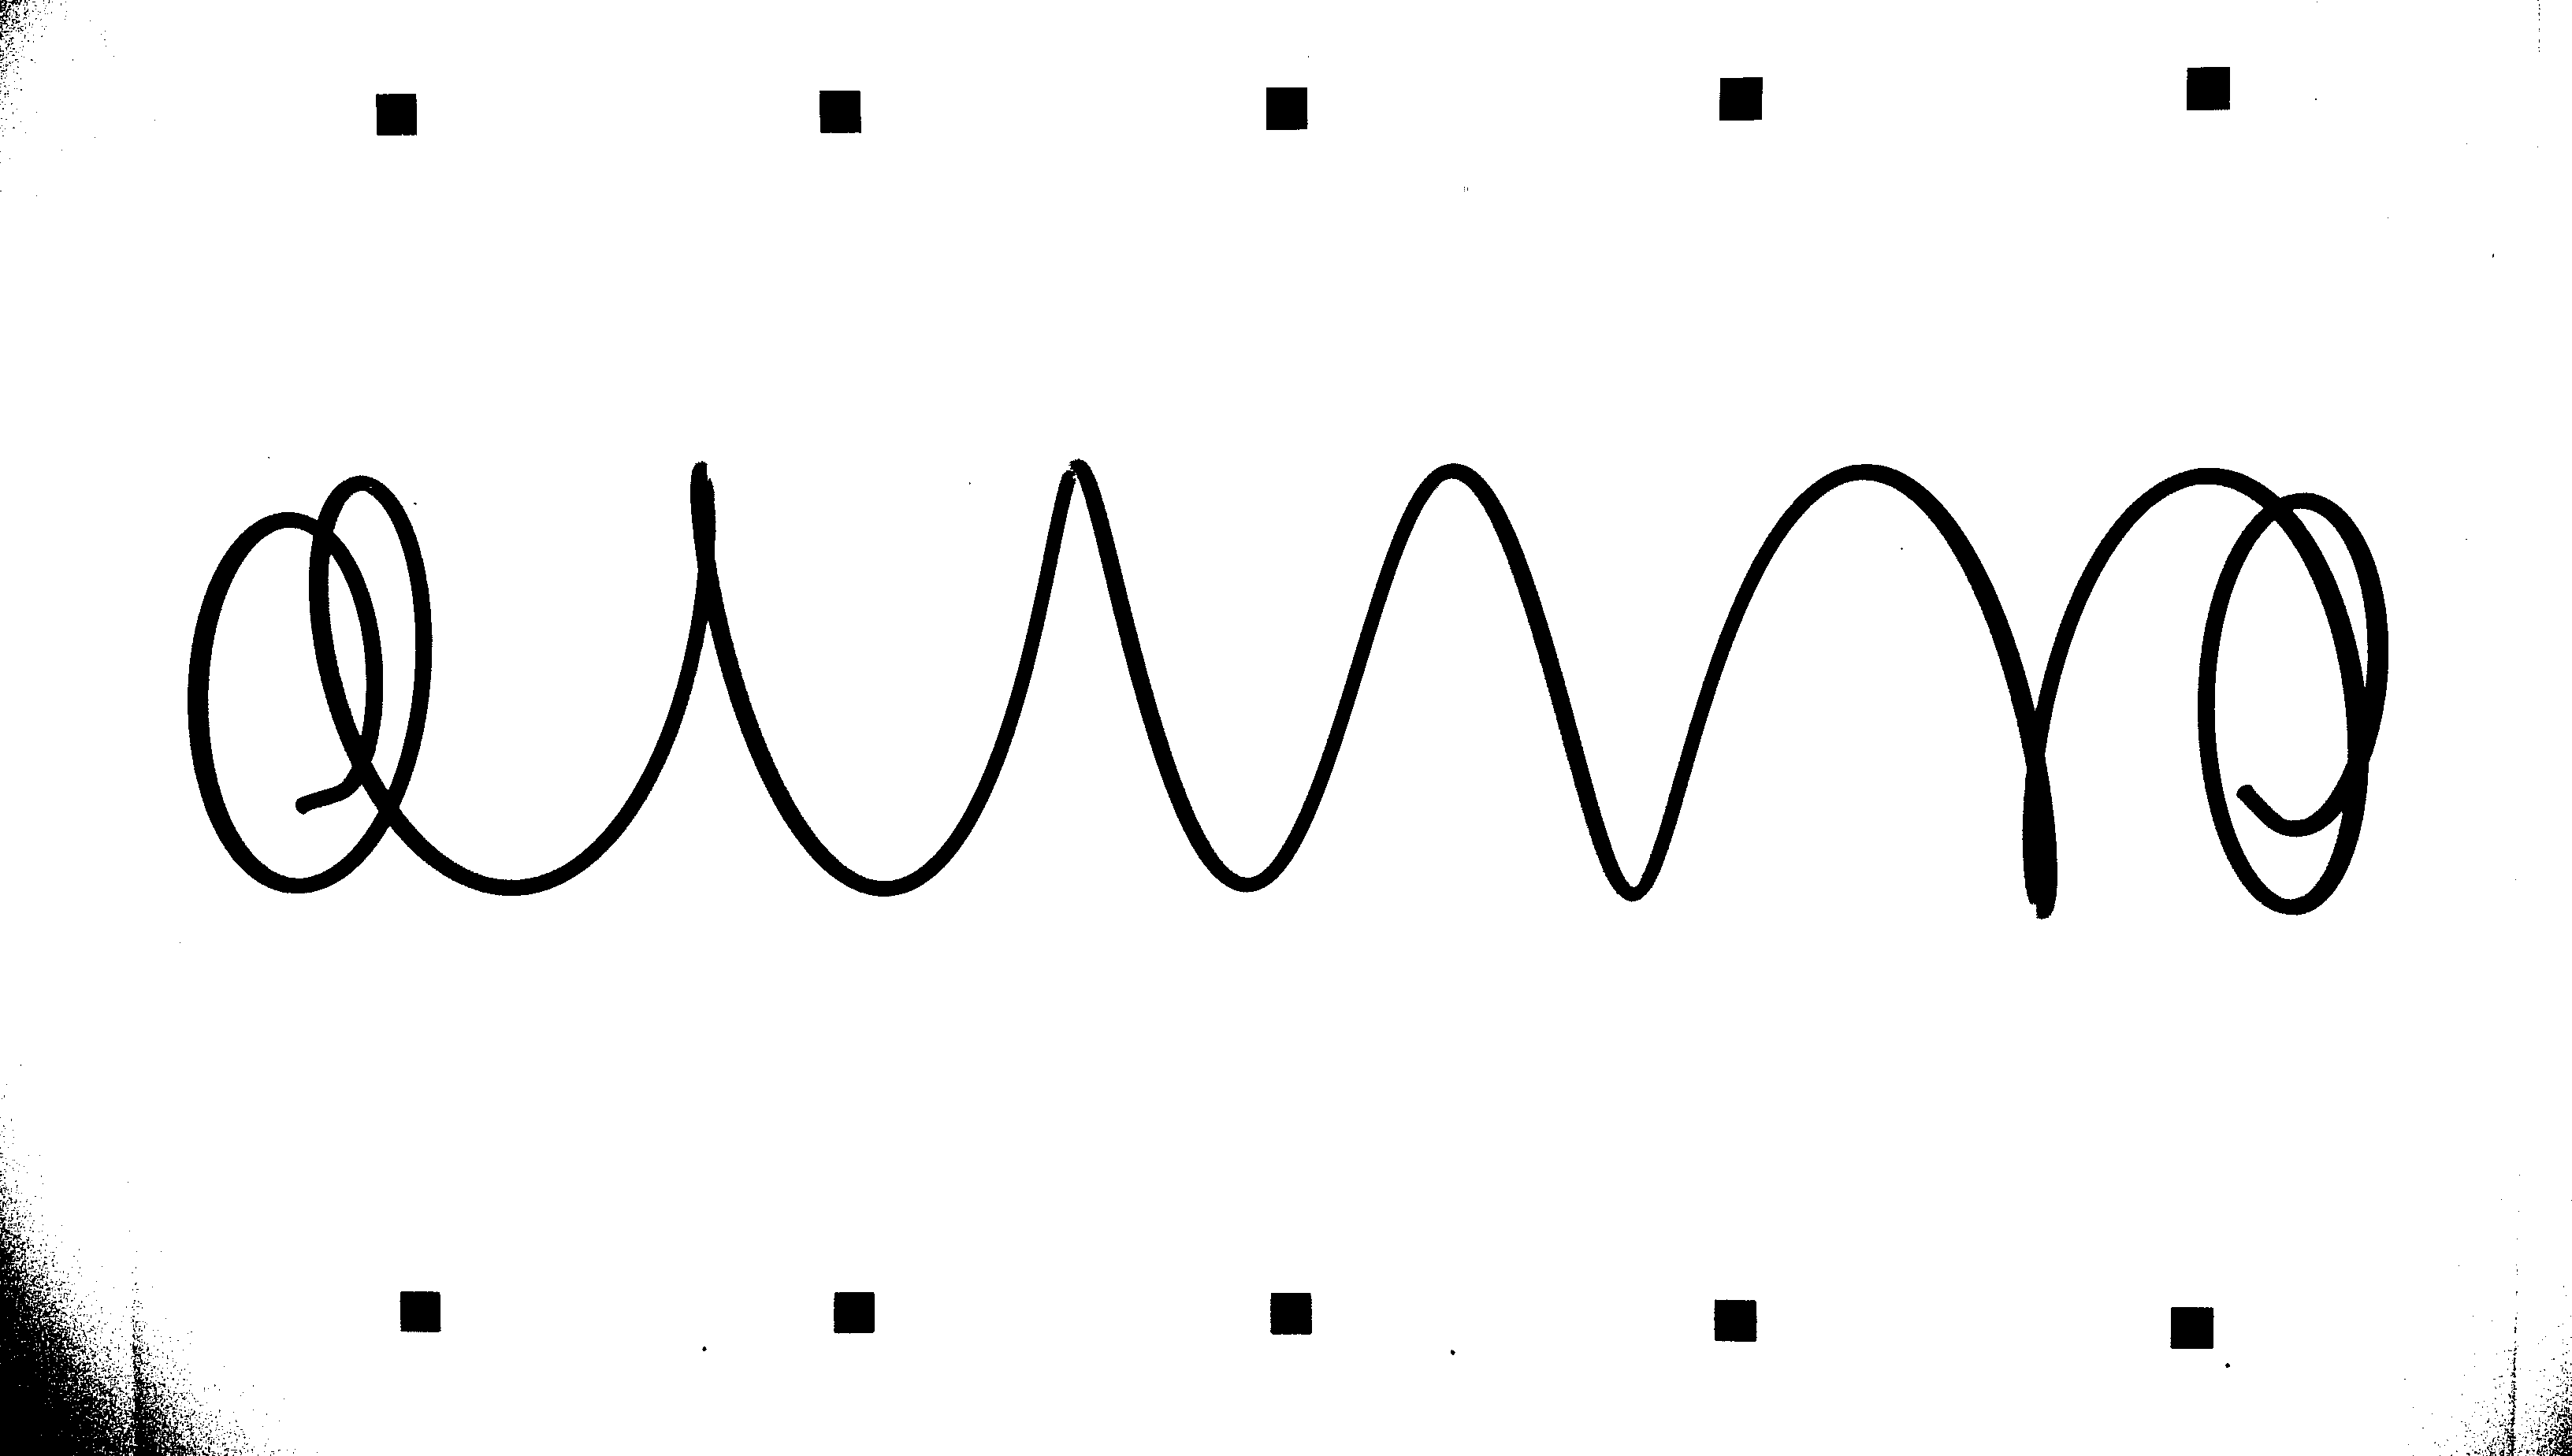
\includegraphics[width=0.45\linewidth, height=5cm]{3-development/threshold/threshold.png}}}
	\subfigure[\label{development:otsu}]{\fbox{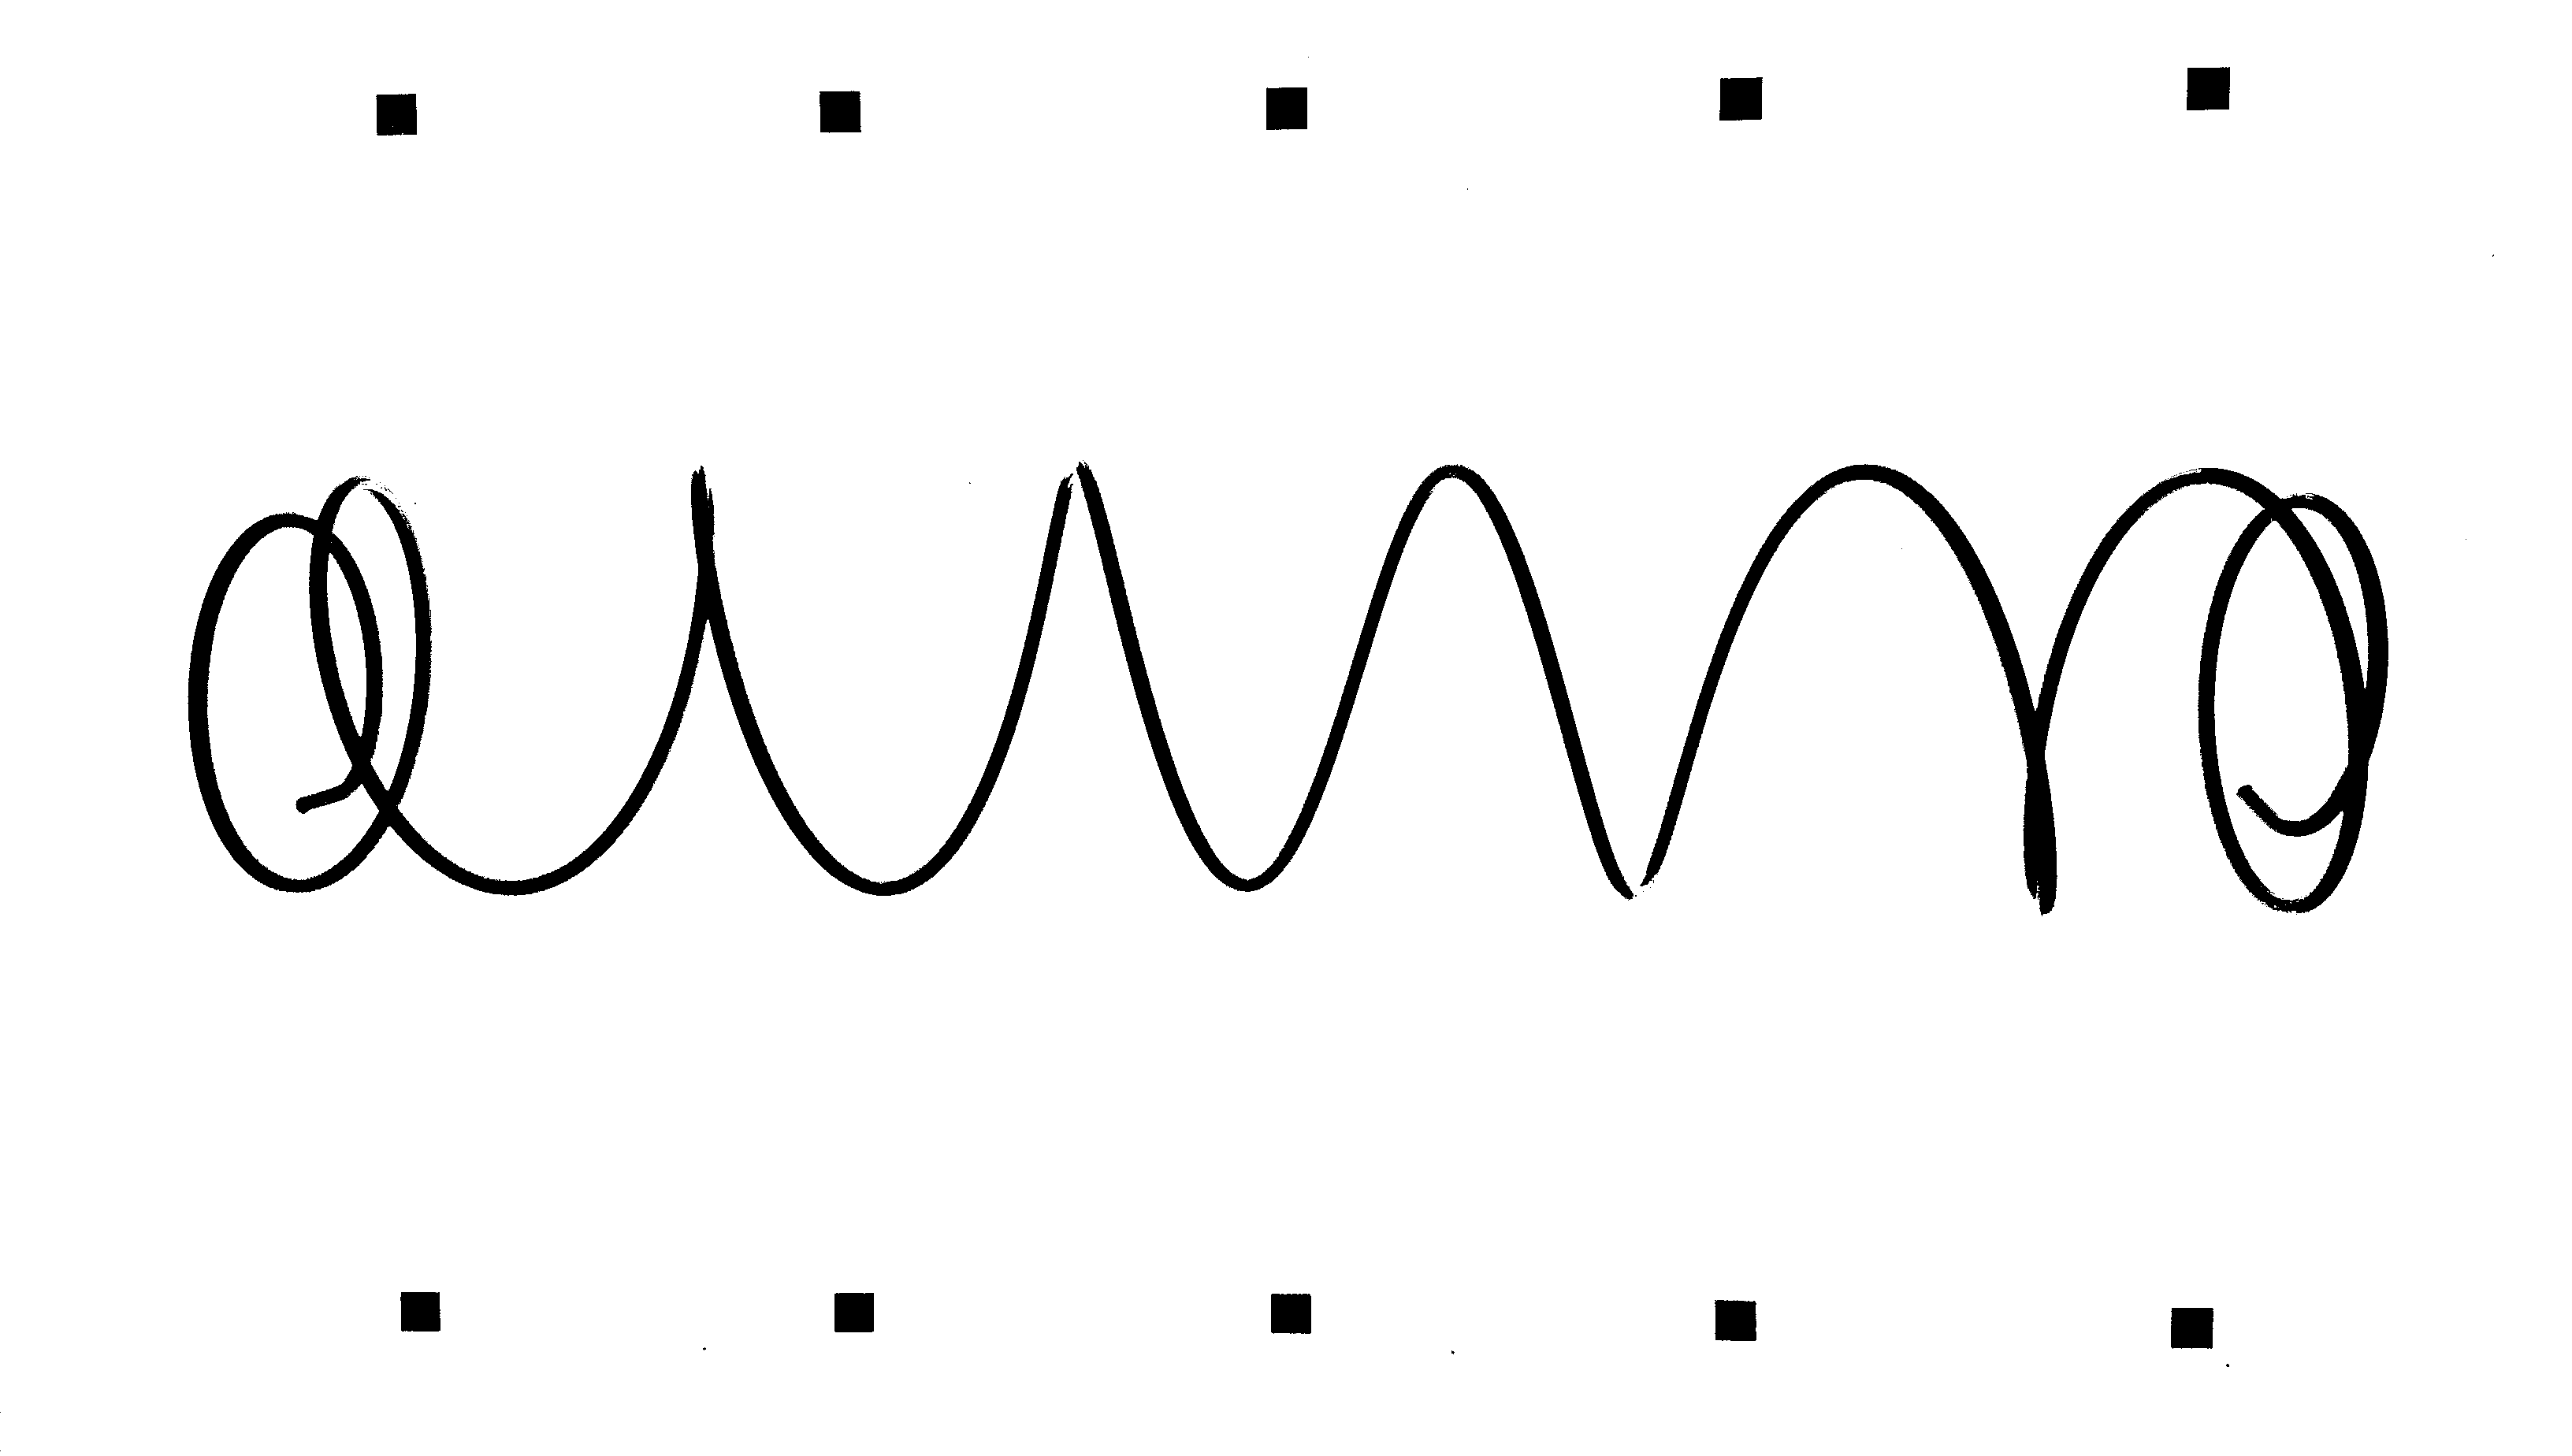
\includegraphics[width=0.45\linewidth, height=5cm]{3-development/threshold/otsu.png}}}
	\subfigure[\label{development:difference}]{\fbox{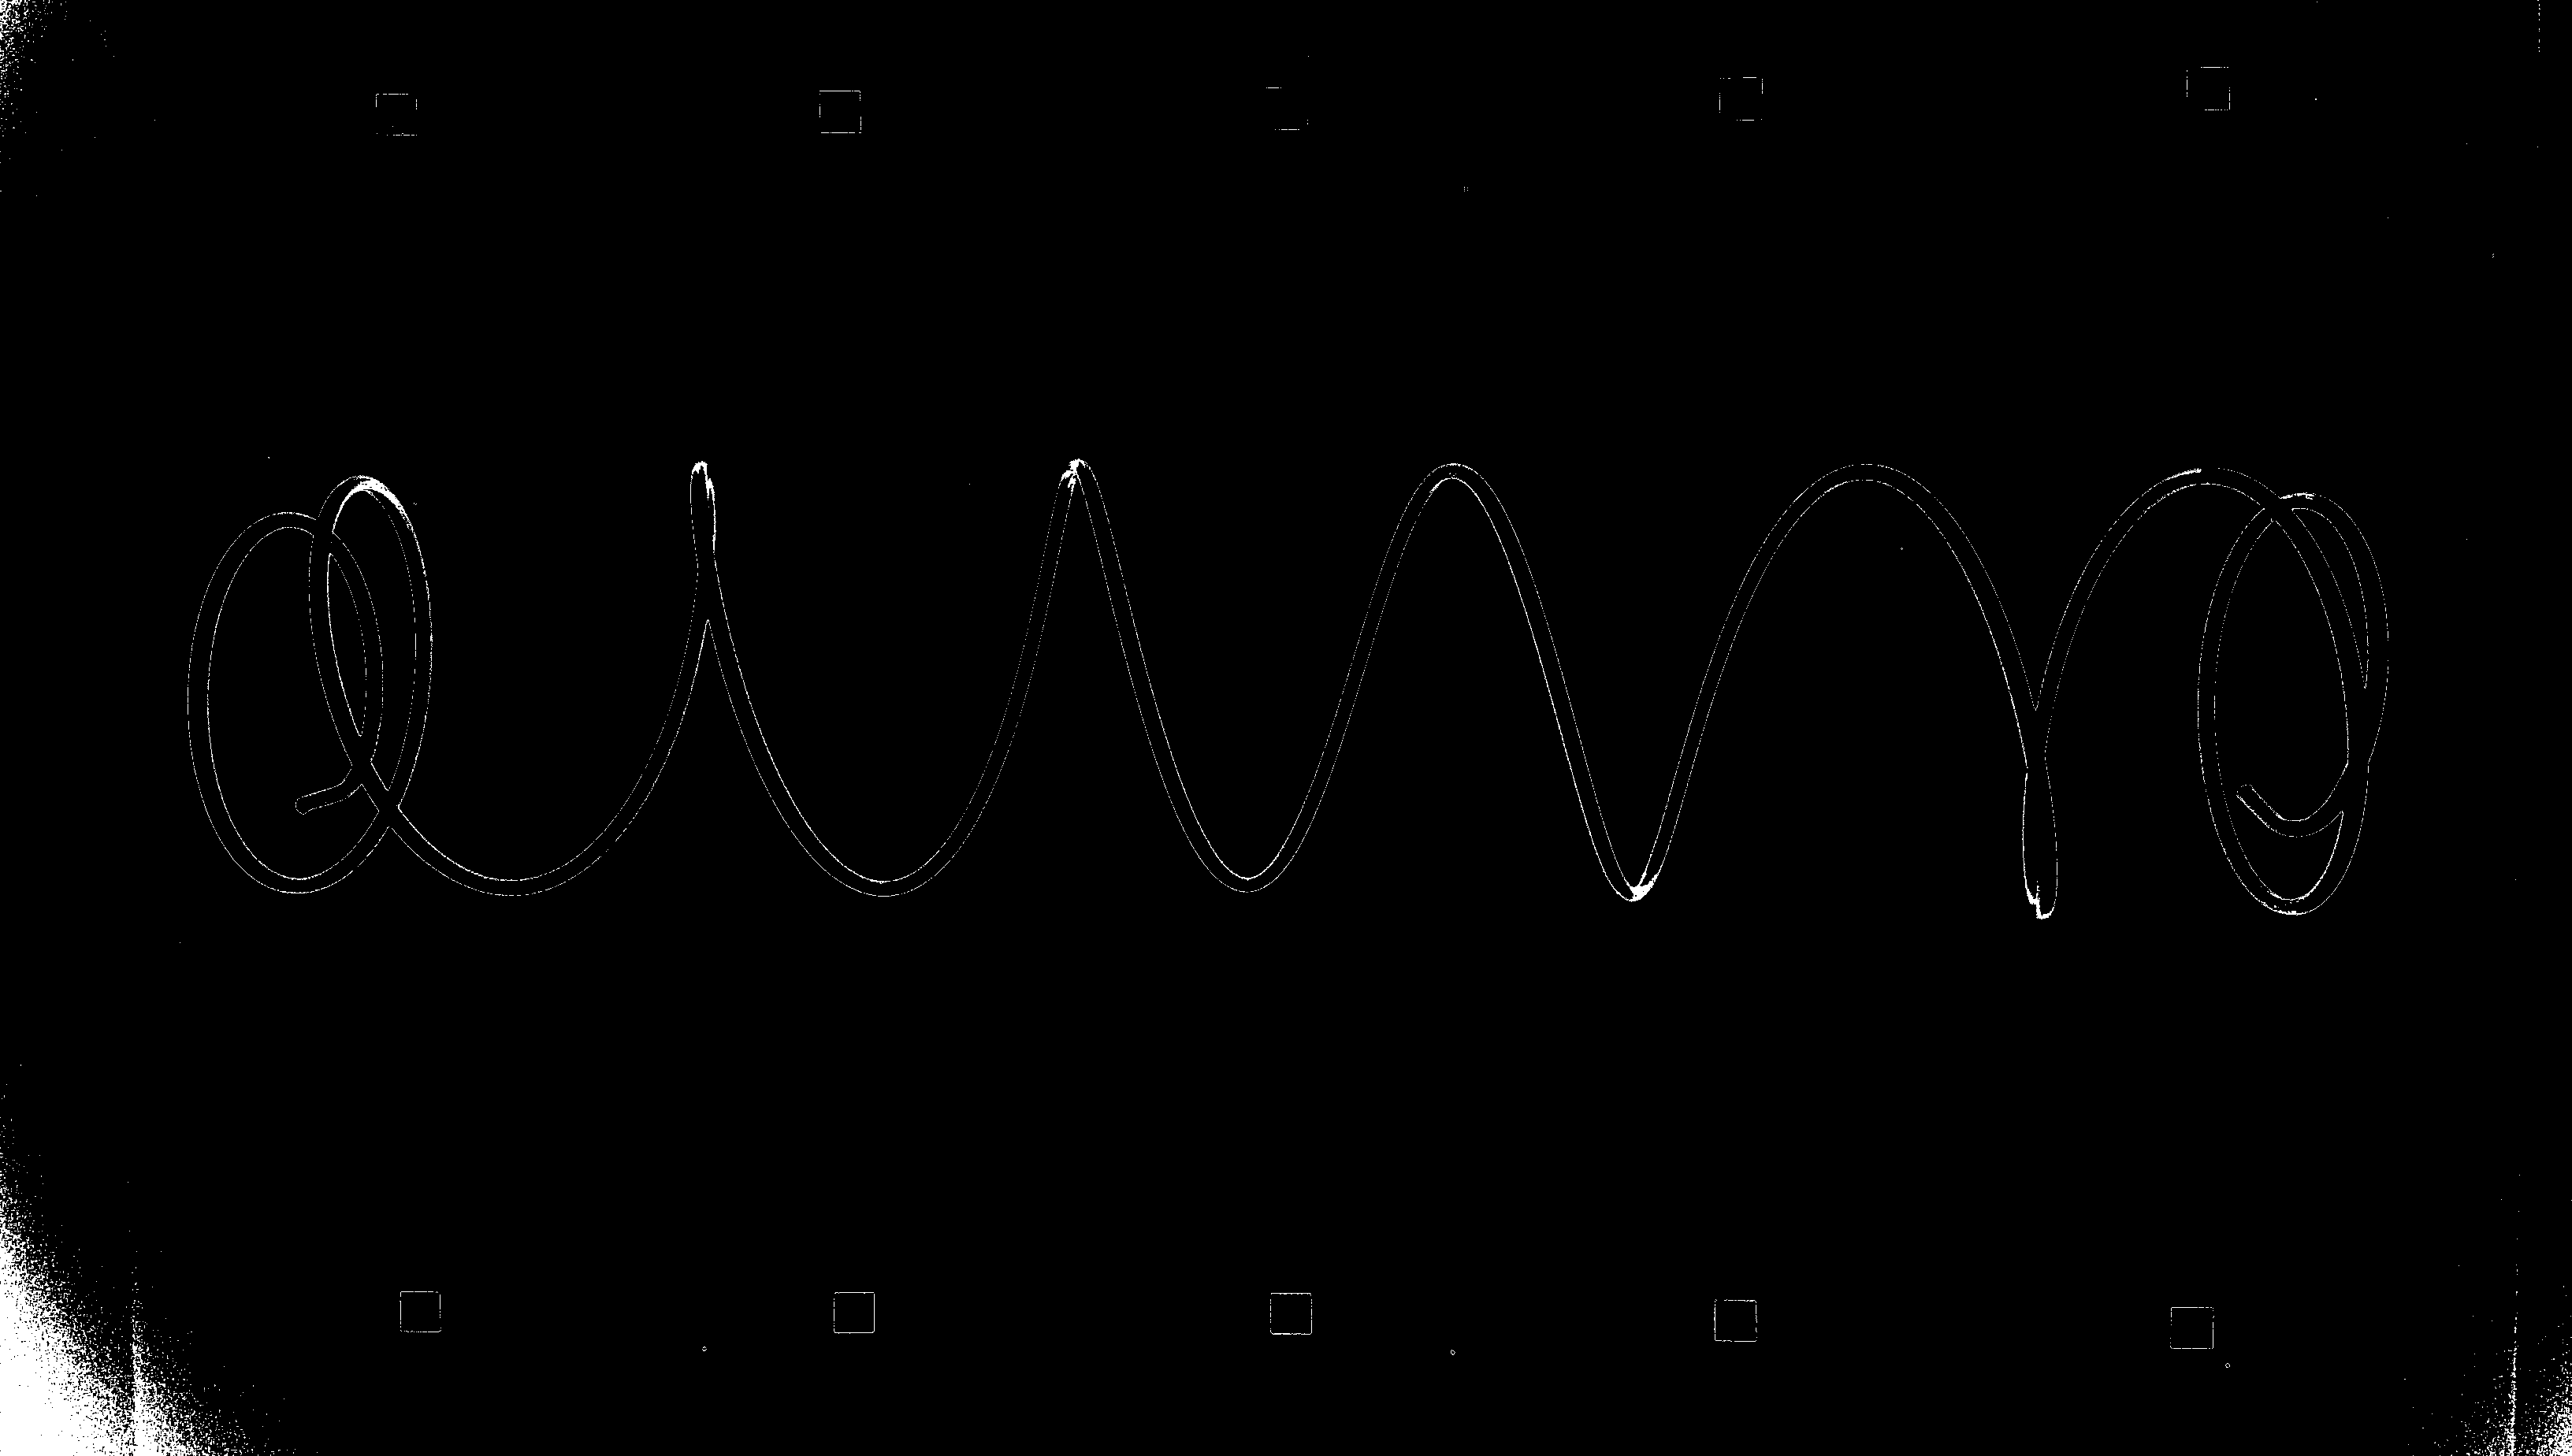
\includegraphics[width=1\linewidth]{3-development/threshold/diff.png}}}
	\caption{Comparison between otsu and triangle threshold\label{development:diff}}	
\end{figure}

If we look closely at the silhouette of the spring after the otsu threshold it seems that in some parts of the spring are disappearing. While the spring in thresholded with the triangle method seems far less effected from this effect. To better illustrate this effect the otsu image is subtracted by the triangle one which results in the difference image \ref{development:difference}.  
Now the difference clearly shows how much information is lost on the edges of the spring and even on the pattern. This information once lost can not be obtained again. With this in mind the otsu seems unsuitable for this problem. \\
The source of the problem itself is that the spring reflects the stray light of the backlight. The stray light is produced by two effects, one is the diffusion film which is only 4mm away from the spring. The second one is the reflected light from the construction itself. Meaning the top of the construction where the camera is mounted reflects some amount back on the spring. These two sources of stray light are leading to the spring being illuminated enough from the top, that some brightness values captured by the camera sensor are the same in the edges of the image as parts of spring.\\
Hardware improvements to minimize this problem would be to use light control filters which results in higher hardware cost. Another way would be to increase the distance between the glass the spring slides over and the diffusion filter so less stray light appears. In additional to these two solution the backlight could be changed so to more LED's in the corner of the PCB. Resulting in a backlight which is brighter in the corners as in the center. While the camera gets less light in the corner called vignetting. This backlight would reduce the vignetting of the camera to a certain amount. \\
Vignetting can also be handled in software. Since the background of the image stays the same it is possible to subtract the background of the image first eliminating the noise in the corner. The down side in correcting the brightness in a complex manner is the time spent doing it. Since every pixel have to be corrected it takes a good amount of time for the whole image. This would reduce the speed of the whole measurement drastically. \\

\subsection{Edge detection}   
To obtain the edge from a thresholded image morphological algorithms are very fast. Thanks to the good threshold results which also uses quite some time to calculate it is now fairly easy to get the edge of the spring. To extract the boundary of the spring we use a 3x3 kernel to erode the given image. The kernel $K$ is shaped as followed:
\begin{center}
\setlength{\tabcolsep}{0.5em} % for the horizontal padding
{\renewcommand{\arraystretch}{1.2}
\begin{tabular}{|c|c|c|}
	\hline
	1&1&1\\
	\hline
	1&1&1\\
	\hline
	1&1&1\\
	\hline
\end{tabular}
}
\end{center}

This kernel $K$ is used to erode the image and subtract the eroded image from the starting image. Lets name the thresholded image $T$. The math done is 
\begin{align*}
 E = T-(T\ominus K)
\end{align*}
returning the image containing all the edges $E$. In our example picture the resulting picture $E$ is displayed in the image \ref{development:edge}.\\



\begin{figure}[!h]
	\centering
	\fbox{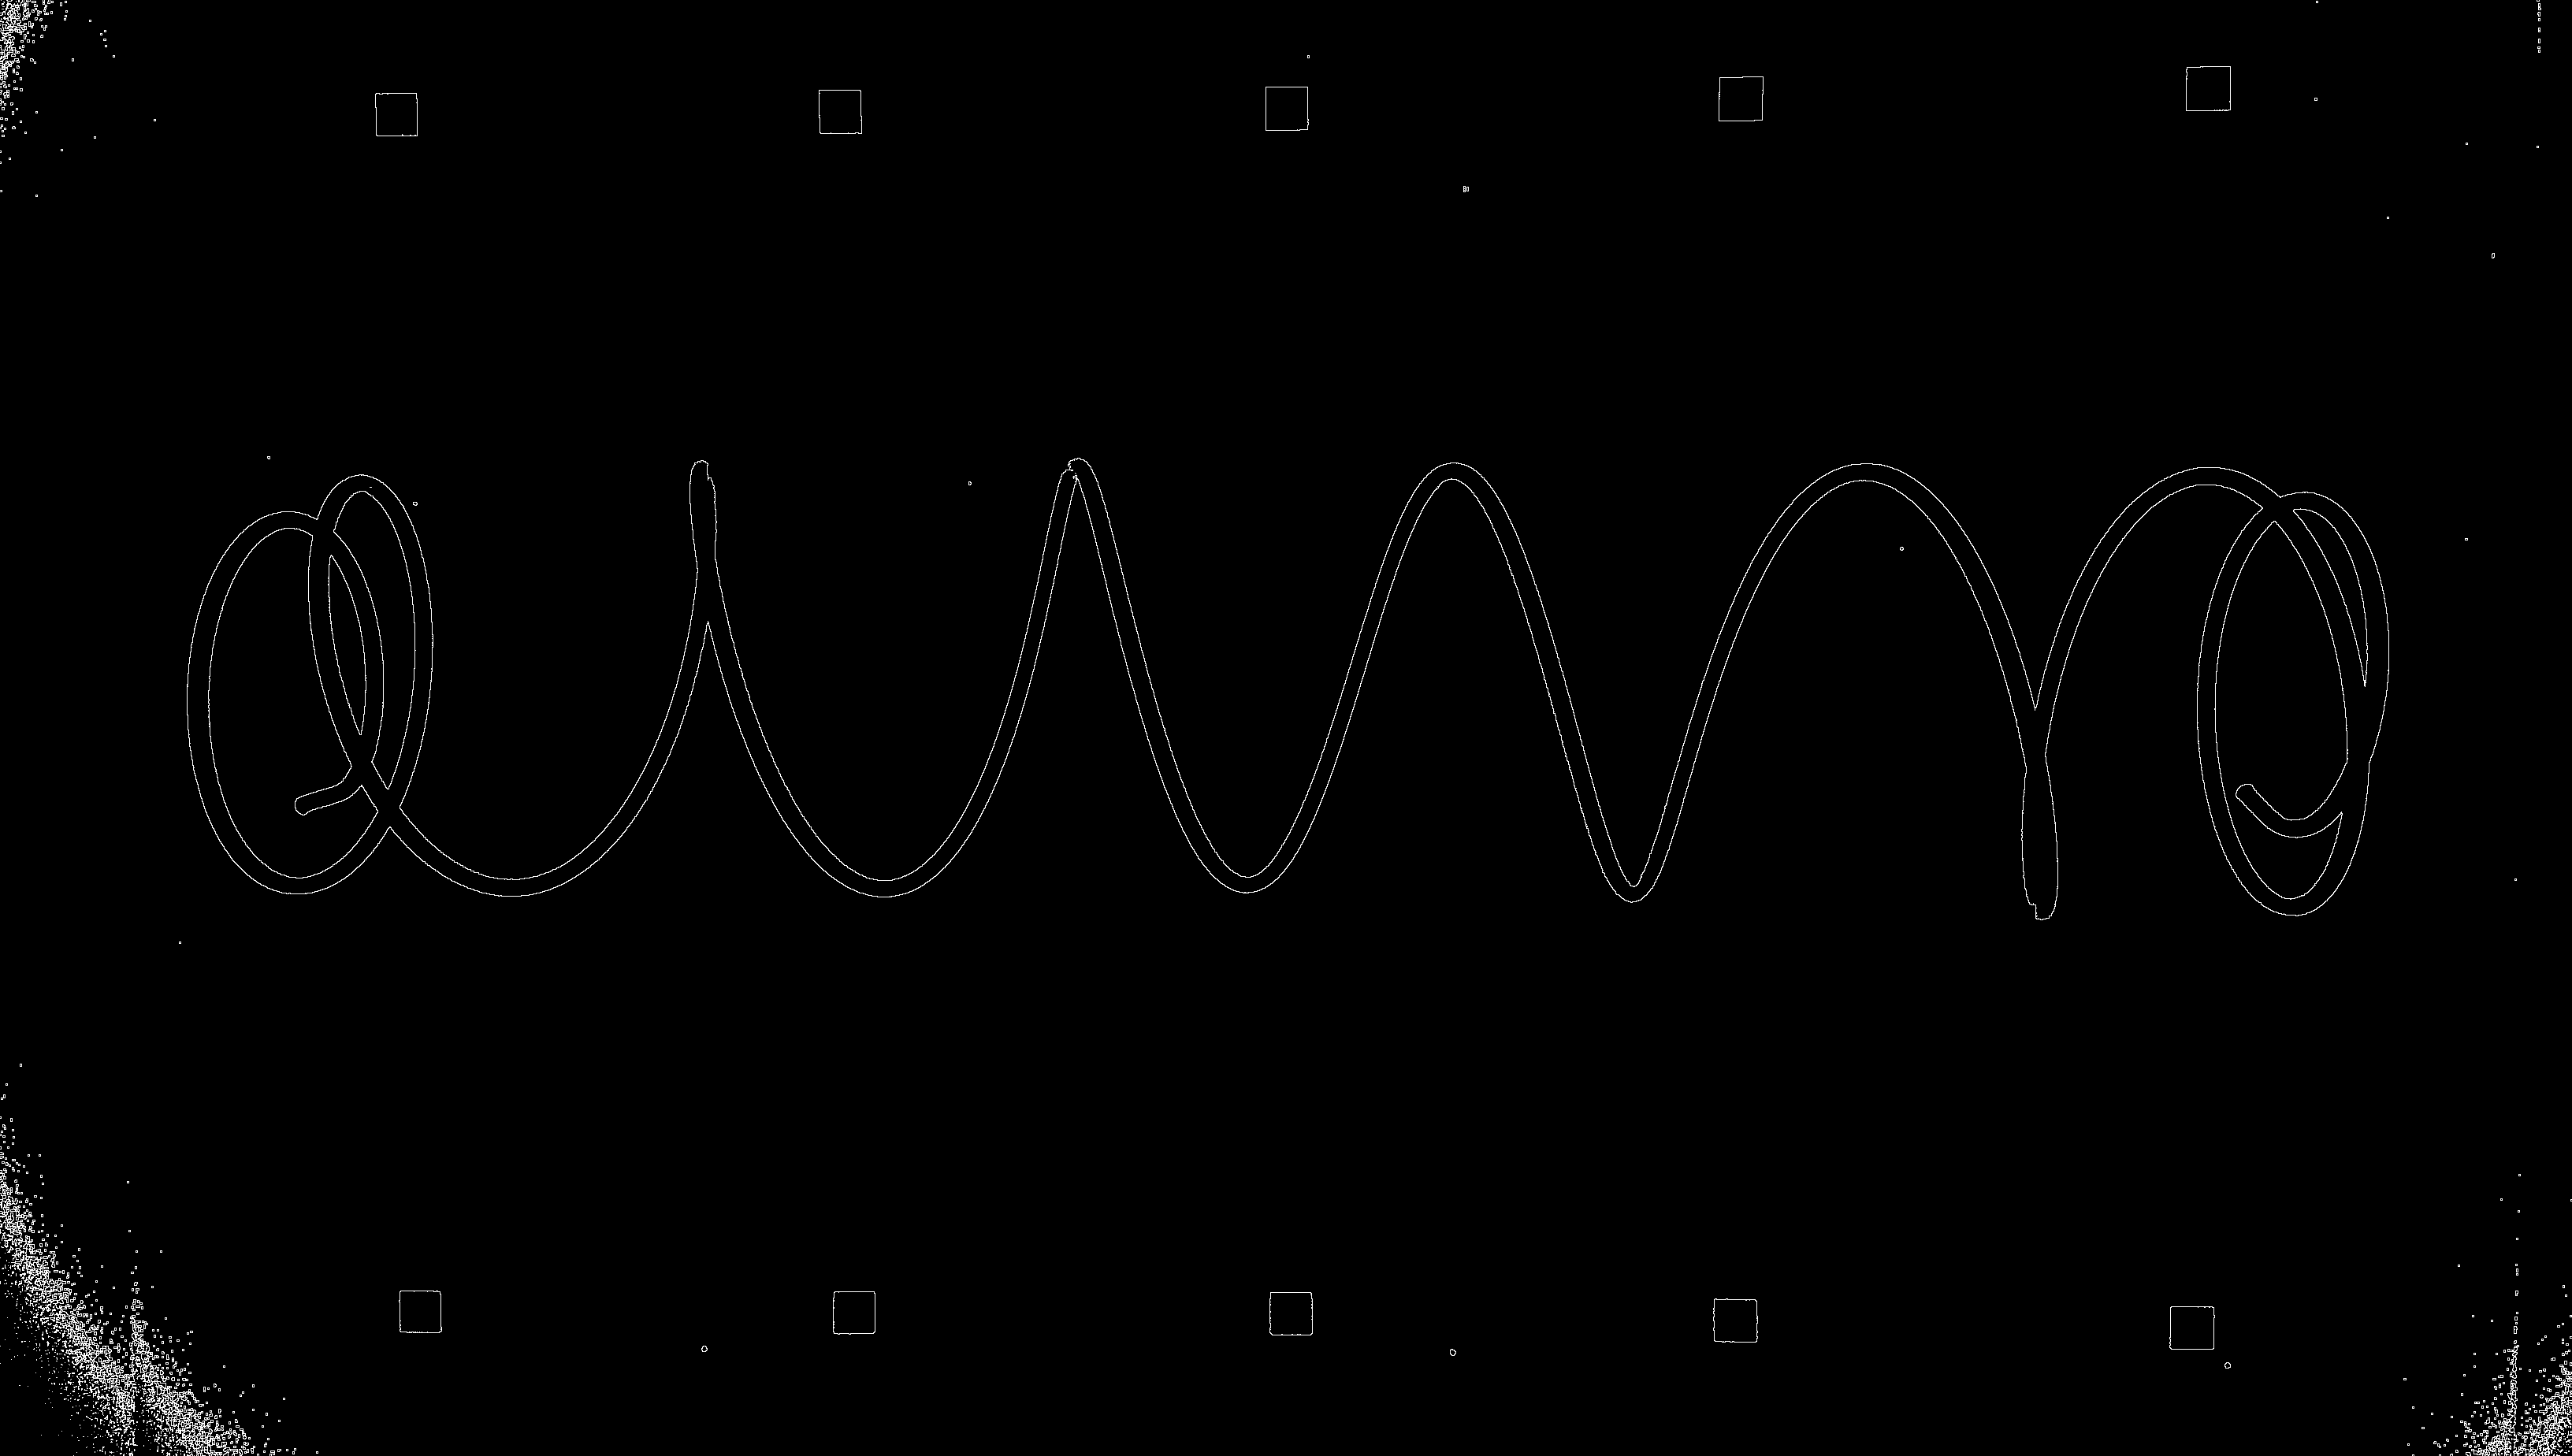
\includegraphics[width=0.9\linewidth]{3-development/threshold/edge.png}}
	\caption{Edges of given image with morphological detection}
	\label{development:edge}
\end{figure}
As we see the image \ref{development:edge} if a noise is bigger than the 3x3 kernel we also receiving the edge of this particular noise. But since we know that our spring cant be located outside of our detection pattern we know we just have to ignore the edges of the image and the small noise in the following steps of calculation.  
\newpage
\section{Software}
To measure an object with a camera, the software has to perform lots of different tasks in a certain period of time.
First off, it needs to take the non linear distortions of the camera into account.
After that, some sort of trigger is needed, to check the frames for objects and pass a frame on, if an object is within the frame.
Now, the software needs to detect a known pattern on the plane where the object lies.
With the known distances of the pattern, a pixel per metric unit can be calculated.
This unit describes, how many pixels in this distance from the camera fit into one metric unit (in this case mm) and is used to convert dimensions in pixel to dimensions in mm and vice versa.
This pattern can also be used to calculate a transformation matrix which compensates for slight angular errors resulting from an imprecise mounting of the camera.
After all these steps, the object has to be recognized.
Finally, the dimensions of the object have to be estimated.

All these steps are described in more detail in the following sections.
For these following sections, it is important to keep in mind, that OpenCV uses a coordinate-system with a switched $x-$ and $y-$axis. 

% listing to python code
\definecolor{codegray}{rgb}{0.5,0.5,0.5}
\definecolor{backcolour}{rgb}{0.95,0.95,0.92}

\lstdefinestyle{mystyle}{
	language=Python,
	backgroundcolor=\color{backcolour},   
	commentstyle=\color{codegreen},
	keywordstyle=\color{blue!50!black},
	numberstyle=\tiny\color{codegray},
	stringstyle=\color{green!50!black},
	basicstyle=\footnotesize\ttfamily,
	breakatwhitespace=false,         
	breaklines=true,                 
	captionpos=b,                    
	keepspaces=true,                 
	numbers=left,                    
	numbersep=2pt,                  
	showspaces=false,                
	showstringspaces=false,
	showtabs=false,                  
	tabsize=2,
	emph={int, char, double, float, range, len, bytes},
	emphstyle=\color{violet},
	morekeywords={as}
}
\lstset{style=mystyle}

\subsection{Initialization}
gobal variables, mapx mapy, init mode

\subsection{Trigger}

\subsection{Edge detection}
morphology

\subsection{Pattern recognition}
The binary image containing the edges is now used to search for the contours of the pattern on the plane.
The pattern consists of 10 rectangles printed on a transparent sheet.
First, it is necessary to find all the contours \texttt{with cv2.findCountours()} inside the two boundaries defined by \texttt{vec} and \texttt{sep}.
This function returns an array of arrays, in which coordinates of the pixels, belonging to one contour are stored.

Because the edge detection is not perfect, some contours will be found which do not belong to the pattern.
By using the area of each contour as basis of decision making, it is possible to remove invalid contours.
This is done in \texttt{remove\_contours()} which is implemented in \texttt{geometry.py}.
If an area of a contour is not between $2600$ and $3400\,$ pixels (both values are passed to the function), the contour is removed.
These two values are of course depended on the rectangle size used and the distance from the camera to the plane.

These left contours (basically an array of points) can be undistorted using \texttt{map\_x} and \texttt{map\_y}.

Now a rectangle is fitted over each contour (with \texttt{cv2.minAreaRect()}).
The center of each rectangle is stored in an array.
These points are here called image-points (in the code as variable \texttt{imgp}).

It is now possible to calculate the pixel per metric unit (\texttt{ppm}) by computing a distance between two image points in pixels and then dividing this distance by the real pattern distance in mm.
In fact it is even more reasonable to do this for a lot of distances and taking the mean of each \texttt{ppm}, assuming that errors in the pattern detection will cancel each other out.

After that, a numpy-array which describes the same pattern how it should appear on the plane if the camera was mounted correctly is generated
This points are here called object-points (\texttt{objp}).
In python this looks like this:
\begin{lstlisting}
	objp = np.array([[-110 * ppm + cx, -75 * ppm + cy],
	                 [ -55 * ppm + cx, -75 * ppm + cy],
	                 [             cx, -75 * ppm + cy],
	                 [  55 * ppm + cx, -75 * ppm + cy],
	                 [ 110 * ppm + cx, -75 * ppm + cy],
	                 [-110 * ppm + cx,  75 * ppm + cy],
	                 [ -55 * ppm + cx,  75 * ppm + cy],
	                 [             cx,  75 * ppm + cy],
	                 [  55 * ppm + cx,  75 * ppm + cy],
	                 [ 110 * ppm + cx,  75 * ppm + cy]], dtype=np.float32)
\end{lstlisting}
where the variables \texttt{cx} and \texttt{cy} are the coordinates of the calibrated principal point of the camera.
The datatype of the entries is forced to float32 because some OpenCV functions do not accept other types.

Now that we have our image- and object points, a perspective transformation matrix can be calculated with
\begin{lstlisting}
	 T, _ = cv2.findHomography(imgp, objp, method=0)
\end{lstlisting}
This function calculates \text{T} in such a way, that the image-points are mapped to the object points using the least-square method (set by \texttt{method=0}).
Or more mathematical:
\begin{align*}
	\begin{pmatrix}
	x_{\text{obj}, i}\\
	y_{\text{obj}, i}\\
	1
	\end{pmatrix}\sim T
	\begin{pmatrix}
	x_{\text{img}, i}\\
	y_{\text{img}, i}\\
	1
	\end{pmatrix}	
\end{align*}
such that
\begin{align*}
	\sum_{i}\left(x_{\text{obj},i}-\frac{T_{11}x_{\text{img},i}+T_{12}y_{\text{img},i}+T_{13}}{T_{31}x_{\text{img},i}+T_{32}y_{\text{img},i}+T_{33}}\right)^2+
	\sum_{i}\left(y_{\text{obj},i}-\frac{T_{21}x_{\text{img},i}+T_{22}y_{\text{img},i}+T_{23}}{T_{31}x_{\text{img},i}+T_{32}y_{\text{img},i}+T_{33}}\right)^2
\end{align*}
is minimized \cite{cv_calib}.
The matrix \texttt{T} is later used to compensate the error made because of the camera mounting. 

\subsection{Object recognition and geometry estimation}
Now that these first calculations are made, the object is detected just like the pattern.
With the function \text{cv2.findcontours()} all contours are extracted from the image with the edges, but this time in between the separation \texttt{sep}.
And again like before, invalid contours are removed, based on their area and undistorted.
because the object in this case is a steel spring, the contours are somewhat complicated and it is possible, that contours are found, which are not connected to each other but definitely belong to the spring.
In this case, the OpenCV function returns them as different contours and it is therefore necessary to combine all returned contours into one single array.
The following code shows how this is achieved in addition with applying the rectification transform and fitting a rectangle over it,
\begin{lstlisting}
	# combine contours to one
	cnts_m = np.concatenate(cnts_m, axis=0).astype(np.float64)
	
	# warp perspective of the contours
	cnts_m = cv2.perspectiveTransform(cnts_m, T)
	
	# minimum area rectangle around cnts_m
	box = cv2.minAreaRect(cnts_m.astype(np.float32))
\end{lstlisting}
where \texttt{cnts\_m} are the contours found previously.
Since now a rectangle with its coordinates is know, everything is ready for the actual geometry estimation.

because no telecentric objective is used, one has to consider, that the cemare looks at the edges of the object in a slight angle.
For simplicity, it is at this point assumed that the steel spring as a cylinder, which is aligned horizontal in the image plane.
A cut through the center of this cylinder along the $y$-axis (OpenCV coordinates) is show in figure \ref{development:diameter}.
\begin{figure}[ht]
	\centering
	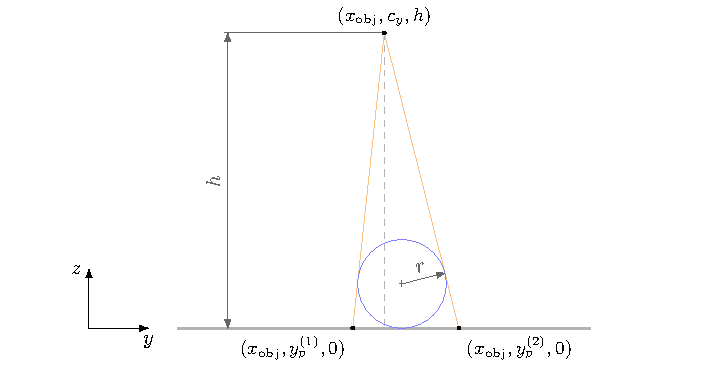
\includegraphics[width=0.9\linewidth]{3-development/software/images/diameter_estimation.pdf}
	\caption{Steel spring cut through the center along $y$-axis\label{development:diameter}}
\end{figure}
$x_{\text{obj}}$ denotes the center of the object (spring) while $cx$ is the $x-$coordinate of the calibrated principal point.
The distance from the camera to the plane can be calculated by using the theorem of intersecting lines, since the focal length and pixel-size are known from the data-sheet of the camera and the pixel per metric unit has been calculated previously.
Also known are the two observed points on the plane $(x_{\text{obj}}, y_p^{(1)})$ and $(x_{\text{obj}}, y_p^{(2)})$.

The distances from these two points on the plane to the camera and to each other can now be calculated as
\begin{align*}
	d_{1}&=\sqrt{(c_y-y_p^{(1)})^2+h^2}\\
	d_{2}&=\sqrt{(c_y-y_p^{(2)})^2+h^2}\\
	d_{3}&=y_p^{(2)}-y_p^{(1)}.
\end{align*}
The distance must of course have the same units, in this case all distances in pixel where first converted to distances in mm.

This provides enough information to apply the geometry of in-circles \cite{incircles} to calculate the radius of the object as
\begin{align*}
	r=\sqrt{\frac{(s-d_1)(s-d_2)(s-d_3)}{s}}
\end{align*}
with
\begin{align*}
	s=\frac{d_1+d_2+d_3}{2}.
\end{align*}

A similar principle is applied to calculate the length of the object.
Figure \ref{development:length} where again
$y_{\text{obj}}$ denotes the center of the object (spring) while $yx$ is the $y-$coordinate of the calibrated principal point.
\begin{figure}[ht]
	\centering
	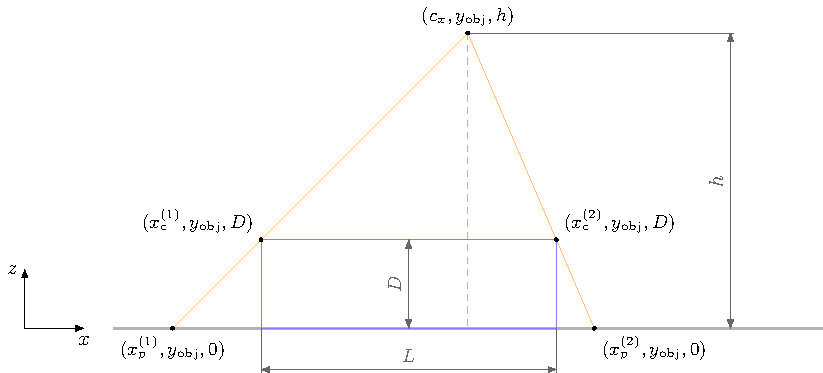
\includegraphics[width=0.9\linewidth]{3-development/software/images/length_estimation.pdf}
	\caption{Steel spring cut through the center along $x$-axis\label{development:length}}
\end{figure}
The points which can be observed in the image are 






\chapter{Results}
This chapter covers the most important results.

\chapter{Conclusion}

\section{Reflection}
A device to demonstrate the measurement of an object with a low-cost optic has been developed.
It could be shown, that with this setup, the relative errors in the measured dimensions can be kept inside a reasonable deviation (max. rel. error = 1.6\%).
The software responsible for the computations is fast enough to deal with the expected 200 springs per minute and the errors caused by the rolling shutter can be compensated in a simple way assuming the object moves horizontal through the frame and has a constant speed which has to be estimated beforehand.

The cost of the whole device could be kept below (999999999 yen).
This lowers the expenditures of a company, using this technology in their production chains dramatically compared to similar optical measurement devices nowadays.

Unfortunately, some problems where caused by the trigger.
In many cases, the object moving with the estimated speed of 2\,m/s is not complete inside the image in the first frame, which activates the trigger.
But in the next frame, to object has already partly moved outside the frame and none of the images can be used for measurements.

\section{Further development}
There are of course a lot of improvements to be made.

In order the get a better absolute precision, the calibration process could be improved by detecting the checkerboard more precise or by using a different calibration pattern.
it should also be possible, to take the complicated geometry of the spring into account, instead of just assuming a cylinder.

Implementing the code in C++ should not only make all the processing faster, but also gives the ability to communicate with the driver of the camera reliably.
This is necessary in order to develop a faster trigger which can work with the full 28\,fps instead of just 20\,fps.




%bibliography
\chapter*{References}
\addcontentsline{toc}{chapter}{References} 
\printbibliography[heading=none]

%Abbildungsverzeichnis
\addcontentsline{toc}{chapter}{List of figures} 
\listoffigures\thispagestyle{fancy}

%Tabellenverzeichnis
\addcontentsline{toc}{chapter}{List of tables} 
\listoftables\thispagestyle{fancy}

\addcontentsline{toc}{chapter}{Statement of Plagiarisms} 
\chapter*{Statement of Plagiarism}
%\textbf{Erkl�rung}\\
We declare that, apart from properly referenced quotations, this report is our
own work and contains no plagiarism; it has not been submitted previously
for any other assessed unit on this or other degree courses.
%Wir erkl�ren hiermit an Eides statt, dass ich die vorliegende Arbeit ohne Benutzung anderer als der angegebenen Hilfsmittel erstellt habe; die aus fremden Quellen direkt oder indirekt �bernommenen Gedanken sind als solche kenntlich gemacht. Die Arbeit wurde bisher in gleicher oder �hnlicher Form keiner anderen Pr�fungsbeh�rde vorgelegt und auch noch nicht ver�ffentlicht.\\
\vspace{0.8cm}\\

\begin{tabular}{l l}
    \textbf{Place} & \textbf{Date} \\
    Rapperswil  & \today
\end{tabular}
\vspace{0.8cm}

\textbf{Signatures}\\
\vspace{1.0cm}

Cedric Renda \hspace{3cm} Manuel Tischhauser

\clearpage



\appendix
\chapter{Partial derivatives of the distortion model\label{app}}
Shown are all partial derivatives of the distortion model in \ref{theory:dist} which are needed to implement the error propagation in subsection \ref{theory:error_propagation}.

\begin{align*}
\frac{\partial x''}{\partial k_1}&=\frac{r^2 x'}{1+k_4 r^2+k_5 r^4+k_6 r^6}&\frac{\partial x''}{\partial p_1}&=2x'y'\\
\frac{\partial x''}{\partial k_2}&=\frac{r^4 x'}{1+k_4 r^2+k_5 r^4+k_6 r^6}&\frac{\partial x''}{\partial p_2}&=r^2+2x'^2\\
\frac{\partial x''}{\partial k_3}&=\frac{r^6 x'}{1+k_4 r^2+k_5 r^4+k_6 r^6}&\frac{\partial x''}{\partial s_1}&=r^2\\
\frac{\partial x''}{\partial k_4}&=-r^2x'\frac{1+k_1 r^2+k_2 r^4+k_3 r^6}{(1+k_4 r^2+k_5 r^4+k_6 r^6)^2}&\frac{\partial x''}{\partial s_2}&=r^4\\
\frac{\partial x''}{\partial k_5}&=-r^4x'\frac{1+k_1 r^2+k_2 r^4+k_3 r^6}{(1+k_4 r^2+k_5 r^4+k_6 r^6)^2}&\frac{\partial x''}{\partial s_3}&=0\\
\frac{\partial x''}{\partial k_6}&=-r^6x'\frac{1+k_1 r^2+k_2 r^4+k_3 r^6}{(1+k_4 r^2+k_5 r^4+k_6 r^6)^2}&\frac{\partial x''}{\partial s_4}&=0\\
\end{align*}

\begin{align*}
\frac{\partial y''}{\partial k_1}&=\frac{r^2 x'}{1+k_4 r^2+k_5 r^4+k_6 r^6}&\frac{\partial y''}{\partial p_1}&=r^2+2y'^2\\
\frac{\partial y''}{\partial k_2}&=\frac{r^4 x'}{1+k_4 r^2+k_5 r^4+k_6 r^6}&\frac{\partial y''}{\partial p_2}&=2x'y'\\
\frac{\partial y''}{\partial k_3}&=\frac{r^6 x'}{1+k_4 r^2+k_5 r^4+k_6 r^6}&\frac{\partial y''}{\partial s_1}&=0\\
\frac{\partial y''}{\partial k_4}&=-r^2x'\frac{1+k_1 r^2+k_2 r^4+k_3 r^6}{(1+k_4 r^2+k_5 r^4+k_6 r^6)^2}&\frac{\partial y''}{\partial s_2}&=0\\
\frac{\partial y''}{\partial k_5}&=-r^4x'\frac{1+k_1 r^2+k_2 r^4+k_3 r^6}{(1+k_4 r^2+k_5 r^4+k_6 r^6)^2}&\frac{\partial y''}{\partial s_3}&=r^2\\
\frac{\partial y''}{\partial k_6}&=-r^6x'\frac{1+k_1 r^2+k_2 r^4+k_3 r^6}{(1+k_4 r^2+k_5 r^4+k_6 r^6)^2}&\frac{\partial y''}{\partial s_4}&=r^4\\
\end{align*}


\chapter{Assignment}

\begin{figure}[H]
	\centering
	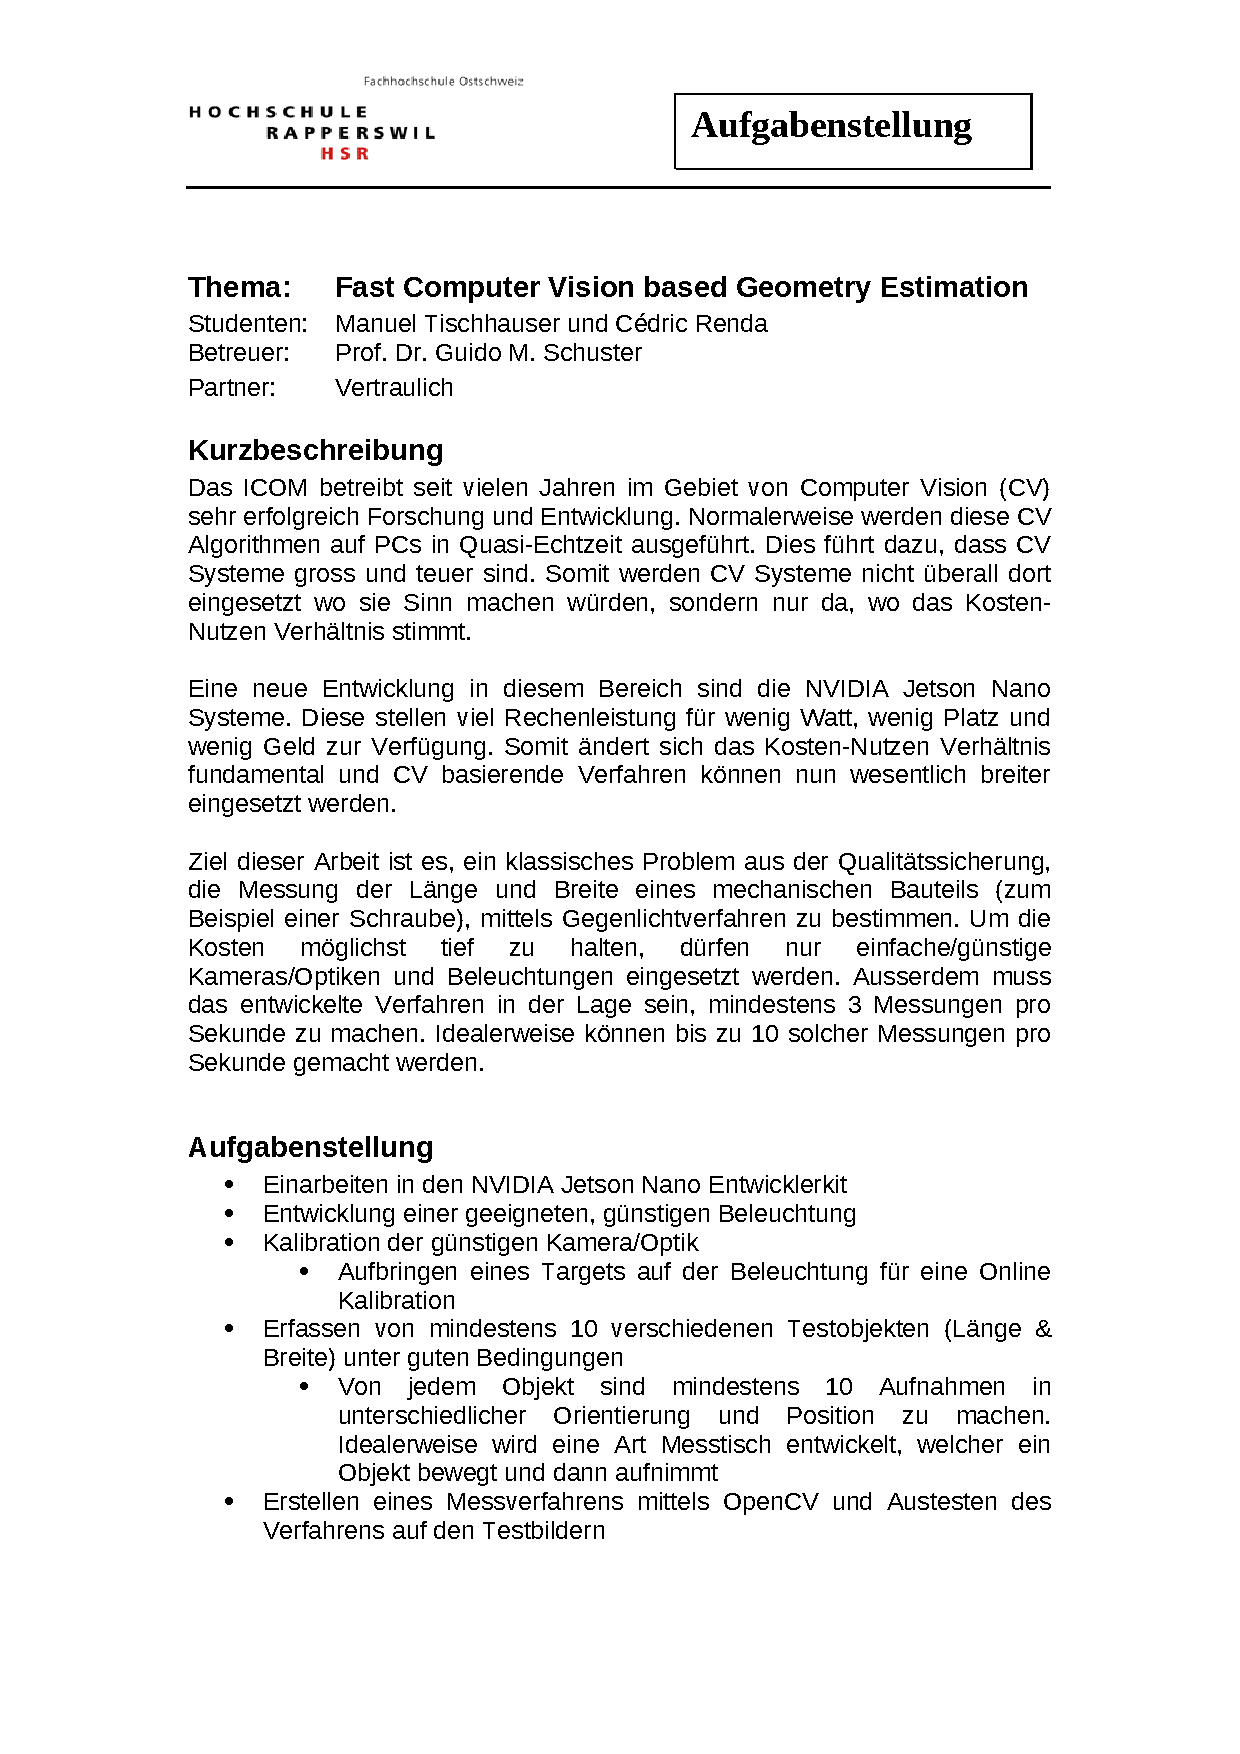
\includegraphics[trim= 0cm 0cm 0cm 0cm,page=1,width=13cm]{FastCVbasedGeometryEstimation.pdf}
\end{figure}
\begin{figure}[H]
	\centering
	\includegraphics[trim= 0cm 0cm 0cm 0cm,page=2,width=13cm]{FastCVbasedGeometryEstimation.pdf}
\end{figure}




\vfill
\pagebreak
\ifodd\value{page}\else\null\clearpage\fi
\lhead{Index}
\rhead{}
\addcontentsline{toc}{chapter}{\indexname}
\input main.ind
\end{document}
